%% 由 build/emit_tex.py 生成（生成物，勿手改）；定制请放 user_style.tex / user_meta.yaml
\chapter{第 7 章 ·
Statsmodels及其基本使用}\label{ux7b2c-7-ux7ae0-statsmodelsux53caux5176ux57faux672cux4f7fux7528}

\section{01
方差分析与回归}\label{ux65b9ux5deeux5206ux6790ux4e0eux56deux5f52}

\begin{quote}
本节对应原版 7.1 的内容，并增补目标、诊断、GLM、WLS 与思考题。
配套图：figures/07-statsmodels/regression\_ols.png、figures/07-statsmodels/anova\_boxes.png、figures/07-statsmodels/qq\_resid.png（由
build/make\_chap7\_figures.py 生成）。
\end{quote}

\subsection{本节目标}\label{ux672cux8282ux76eeux6807-26}

\begin{itemize}
\tightlist
\item
  会用 statsmodels.api.OLS 与 add\_constant 做一元/多元线性回归，并读懂
  summary()；
\item
  会用公式 API ols(`y \textasciitilde{} x', data=df)，理解分类变量
  C(\ldots) 与交互项写法；
\item
  会用 anova\_lm 做单因素方差分析，解读 F 统计量与 P 值；
\item
  会用 GLM + Binomial 做二分类 Logit 回归并得到概率；
\item
  会做基本回归诊断（残差 QQ 图、JB 统计量）与异方差处理（WLS）。
\end{itemize}

\subsection{先修}\label{ux5148ux4fee-19}

\begin{itemize}
\tightlist
\item
  Python 基础、NumPy 数组、Pandas
  DataFrame；了解最小二乘与回归的统计含义。
\item
  已安装 statsmodels（见章 README）。
\end{itemize}

\subsection{官方文档/参考入口}\label{ux5b98ux65b9ux6587ux6863ux53c2ux8003ux5165ux53e3-5}

{\def\LTcaptype{none} % do not increment counter
\begin{longtable}[]{@{}
  >{\raggedright\arraybackslash}p{(\linewidth - 4\tabcolsep) * \real{0.3333}}
  >{\raggedright\arraybackslash}p{(\linewidth - 4\tabcolsep) * \real{0.3333}}
  >{\raggedright\arraybackslash}p{(\linewidth - 4\tabcolsep) * \real{0.3333}}@{}}
\toprule\noalign{}
\begin{minipage}[b]{\linewidth}\raggedright
内容
\end{minipage} & \begin{minipage}[b]{\linewidth}\raggedright
链接
\end{minipage} & \begin{minipage}[b]{\linewidth}\raggedright
说明
\end{minipage} \\
\midrule\noalign{}
\endhead
\bottomrule\noalign{}
\endlastfoot
OLS（回归模型） &
\href{https://www.statsmodels.org/stable/generated/statsmodels.regression.linear_model.OLS.html}{链接}
& 最小二乘回归主接口 \\
Regressions 官方教程 &
\href{https://www.statsmodels.org/stable/regression.html}{链接} &
回归模型总览 \\
公式 API & \href{https://www.statsmodels.org/stable/formula.html}{链接}
& ols(`y \textasciitilde{} x', data=\ldots) 语法 \\
anova\_lm &
\href{https://www.statsmodels.org/stable/generated/statsmodels.stats.anova.anova_lm.html}{链接}
& 对 OLS 结果做方差分析 \\
GLM &
\href{https://www.statsmodels.org/stable/generated/statsmodels.genmod.generalized_linear_model.GLM.html}{链接}
& 广义线性模型 \\
WLS &
\href{https://www.statsmodels.org/stable/generated/statsmodels.regression.linear_model.WLS.html}{链接}
& 加权最小二乘 \\
\end{longtable}
}

\begin{center}\rule{0.5\linewidth}{0.5pt}\end{center}

\subsection{1 方差分析（ANOVA）}\label{ux65b9ux5deeux5206ux6790anova}

\subsubsection{1.1 概念}\label{ux6982ux5ff5}

方差分析（ANOVA, Analysis of
Variance）用来检验\textbf{多个组的均值是否显著不同}。其核心思路是把总离差平方和
\(SS_{tot}\) 分解为\textbf{组间平方和} \(SS_{between}\)
与\textbf{组内平方和} \(SS_{within}\)，并构造 F 统计量：

\[
F = \frac{SS_{between}/(k-1)}{SS_{within}/(N-k)}
\]

其中 \(k\) 为组数，\(N\) 为总样本数。若 \(F\) 很大（对应 P
值很小），说明组间差异显著，各组的总体均值不全相等。

Statsmodels 通常先用 OLS
拟合一个``将分组变量视为分类自变量''的模型，再用 anova\_lm
输出方差分析表。

\subsubsection{1.2
单因素方差分析示例}\label{ux5355ux56e0ux7d20ux65b9ux5deeux5206ux6790ux793aux4f8b}

构造三个组（A/B/C），每组均值分别为 0、1、2，并加噪声：

\begin{Shaded}
\begin{Highlighting}[]
\ImportTok{import}\NormalTok{ numpy }\ImportTok{as}\NormalTok{ np}
\ImportTok{import}\NormalTok{ pandas }\ImportTok{as}\NormalTok{ pd}
\ImportTok{import}\NormalTok{ statsmodels.api }\ImportTok{as}\NormalTok{ sm}
\ImportTok{from}\NormalTok{ statsmodels.formula.api }\ImportTok{import}\NormalTok{ ols}
\ImportTok{import}\NormalTok{ matplotlib.pyplot }\ImportTok{as}\NormalTok{ plt}

\NormalTok{plt.rcParams[}\StringTok{\textquotesingle{}font.sans{-}serif\textquotesingle{}}\NormalTok{] }\OperatorTok{=}\NormalTok{ [}\StringTok{\textquotesingle{}Microsoft YaHei\textquotesingle{}}\NormalTok{, }\StringTok{\textquotesingle{}SimHei\textquotesingle{}}\NormalTok{, }\StringTok{\textquotesingle{}DejaVu Sans\textquotesingle{}}\NormalTok{]}
\NormalTok{plt.rcParams[}\StringTok{\textquotesingle{}axes.unicode\_minus\textquotesingle{}}\NormalTok{] }\OperatorTok{=} \VariableTok{False}

\NormalTok{rng }\OperatorTok{=}\NormalTok{ np.random.default\_rng(}\DecValTok{1}\NormalTok{)}
\NormalTok{n }\OperatorTok{=} \DecValTok{12}
\NormalTok{df }\OperatorTok{=}\NormalTok{ pd.DataFrame(\{}
    \StringTok{\textquotesingle{}group\textquotesingle{}}\NormalTok{: [}\StringTok{\textquotesingle{}A\textquotesingle{}}\NormalTok{]}\OperatorTok{*}\NormalTok{n }\OperatorTok{+}\NormalTok{ [}\StringTok{\textquotesingle{}B\textquotesingle{}}\NormalTok{]}\OperatorTok{*}\NormalTok{n }\OperatorTok{+}\NormalTok{ [}\StringTok{\textquotesingle{}C\textquotesingle{}}\NormalTok{]}\OperatorTok{*}\NormalTok{n,}
    \StringTok{\textquotesingle{}y\textquotesingle{}}\NormalTok{: np.r\_[rng.normal(}\DecValTok{0}\NormalTok{,}\DecValTok{1}\NormalTok{,n), rng.normal(}\DecValTok{1}\NormalTok{,}\DecValTok{1}\NormalTok{,n), rng.normal(}\DecValTok{2}\NormalTok{,}\DecValTok{1}\NormalTok{,n)]}
\NormalTok{\})}
\BuiltInTok{print}\NormalTok{(df.groupby(}\StringTok{\textquotesingle{}group\textquotesingle{}}\NormalTok{)[}\StringTok{\textquotesingle{}y\textquotesingle{}}\NormalTok{].mean().}\BuiltInTok{round}\NormalTok{(}\DecValTok{4}\NormalTok{))}

\NormalTok{model }\OperatorTok{=}\NormalTok{ ols(}\StringTok{\textquotesingle{}y \textasciitilde{} C(group)\textquotesingle{}}\NormalTok{, data}\OperatorTok{=}\NormalTok{df).fit()}
\NormalTok{anova\_res }\OperatorTok{=}\NormalTok{ sm.stats.anova\_lm(model, typ}\OperatorTok{=}\DecValTok{1}\NormalTok{)}
\BuiltInTok{print}\NormalTok{(anova\_res)}
\end{Highlighting}
\end{Shaded}

运行结果：

\begin{Shaded}
\begin{Highlighting}[]
\NormalTok{group}
\NormalTok{A    0.2354}
\NormalTok{B    0.9966}
\NormalTok{C    1.9345}
\NormalTok{Name: y, dtype: float64}

\NormalTok{            df     sum\_sq   mean\_sq         F    PR(\textgreater{}F)}
\NormalTok{C(group)   2.0  17.386102  8.693051  9.297656  0.000627}
\NormalTok{Residual  33.0  30.854088  0.934972       NaN       NaN}
\end{Highlighting}
\end{Shaded}

\begin{figure}
\centering
\pandocbounded{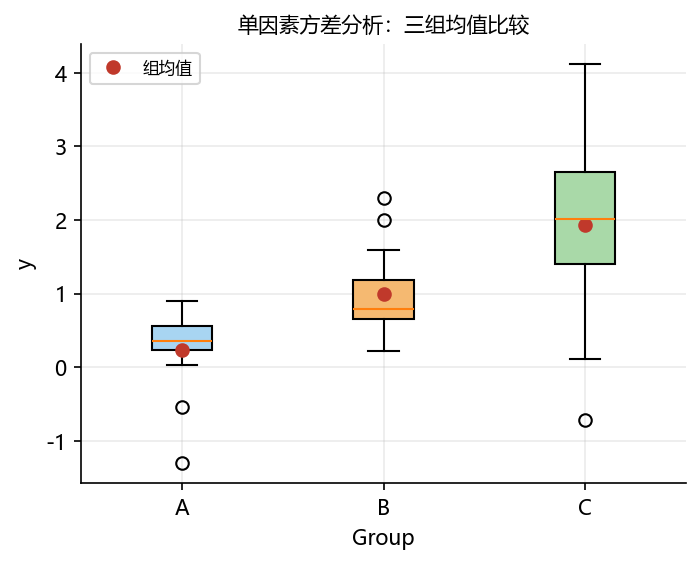
\includegraphics[keepaspectratio,alt={三个组的箱线图}]{figures/07-statsmodels/anova_boxes.png}}
\caption{三个组的箱线图}
\end{figure}

\subsubsection{1.3 解读}\label{ux89e3ux8bfb}

\begin{itemize}
\tightlist
\item
  C(group) 告诉 ols 把 group 当作\textbf{分类变量}，展开成虚拟变量；
\item
  PR(\textgreater F) 是 F 检验的 P 值，本例 0.000627 \textless{}
  0.05，说明三组均值\textbf{存在显著差异}；
\item
  sum\_sq 是平方和，mean\_sq = sum\_sq / df，F = 组间 mean\_sq / 组内
  mean\_sq。
\end{itemize}

\begin{quote}
多做几组对比时，anova\_lm 的 typ 可切换 I/II/III
型平方和；单因素情形三者等价。
\end{quote}

\subsection{案例卡
1：单因素方差分析------三种肥料对产量差异是否显著}\label{ux6848ux4f8bux5361-1ux5355ux56e0ux7d20ux65b9ux5deeux5206ux6790ux4e09ux79cdux80a5ux6599ux5bf9ux4ea7ux91cfux5deeux5f02ux662fux5426ux663eux8457}

\subsubsection{目标}\label{ux76eeux6807-27}

在田间试验里，把同一作物种在 45 块小地上，分别施 A、B、C
三种肥料，每种肥料 15
块地，记录每块地产量。我们要用\textbf{单因素方差分析}（One-Way
ANOVA）回答：三种肥料的平均产量差异，究竟是\textbf{真实的处理效应}，还是\textbf{抽样噪声}造成的巧合。核心统计量是
F 值与其 P 值。

\subsubsection{代码}\label{ux4ee3ux7801-28}

\begin{Shaded}
\begin{Highlighting}[]
\ImportTok{import}\NormalTok{ numpy }\ImportTok{as}\NormalTok{ np}
\ImportTok{import}\NormalTok{ pandas }\ImportTok{as}\NormalTok{ pd}
\ImportTok{import}\NormalTok{ statsmodels.api }\ImportTok{as}\NormalTok{ sm}
\ImportTok{from}\NormalTok{ statsmodels.formula.api }\ImportTok{import}\NormalTok{ ols}
\ImportTok{import}\NormalTok{ matplotlib.pyplot }\ImportTok{as}\NormalTok{ plt}
\ImportTok{import}\NormalTok{ os}

\NormalTok{plt.rcParams[}\StringTok{\textquotesingle{}font.sans{-}serif\textquotesingle{}}\NormalTok{] }\OperatorTok{=}\NormalTok{ [}\StringTok{\textquotesingle{}Microsoft YaHei\textquotesingle{}}\NormalTok{, }\StringTok{\textquotesingle{}SimHei\textquotesingle{}}\NormalTok{, }\StringTok{\textquotesingle{}DejaVu Sans\textquotesingle{}}\NormalTok{]}
\NormalTok{plt.rcParams[}\StringTok{\textquotesingle{}axes.unicode\_minus\textquotesingle{}}\NormalTok{] }\OperatorTok{=} \VariableTok{False}
\NormalTok{np.set\_printoptions(precision}\OperatorTok{=}\DecValTok{4}\NormalTok{, suppress}\OperatorTok{=}\VariableTok{True}\NormalTok{)}
\NormalTok{pd.set\_option(}\StringTok{\textquotesingle{}display.width\textquotesingle{}}\NormalTok{, }\DecValTok{100}\NormalTok{)}

\NormalTok{rng }\OperatorTok{=}\NormalTok{ np.random.default\_rng(}\DecValTok{42}\NormalTok{)}
\NormalTok{n }\OperatorTok{=} \DecValTok{15}
\NormalTok{a }\OperatorTok{=}\NormalTok{ rng.normal(}\DecValTok{50}\NormalTok{, }\DecValTok{6}\NormalTok{, n)}
\NormalTok{b }\OperatorTok{=}\NormalTok{ rng.normal(}\DecValTok{55}\NormalTok{, }\DecValTok{6}\NormalTok{, n)}
\NormalTok{c }\OperatorTok{=}\NormalTok{ rng.normal(}\DecValTok{60}\NormalTok{, }\DecValTok{6}\NormalTok{, n)}
\NormalTok{df }\OperatorTok{=}\NormalTok{ pd.DataFrame(\{}\StringTok{\textquotesingle{}fertilizer\textquotesingle{}}\NormalTok{: [}\StringTok{\textquotesingle{}A\textquotesingle{}}\NormalTok{]}\OperatorTok{*}\NormalTok{n }\OperatorTok{+}\NormalTok{ [}\StringTok{\textquotesingle{}B\textquotesingle{}}\NormalTok{]}\OperatorTok{*}\NormalTok{n }\OperatorTok{+}\NormalTok{ [}\StringTok{\textquotesingle{}C\textquotesingle{}}\NormalTok{]}\OperatorTok{*}\NormalTok{n,}
                   \StringTok{\textquotesingle{}out\textquotesingle{}}\NormalTok{: np.r\_[a, b, c]\})}

\BuiltInTok{print}\NormalTok{(df.groupby(}\StringTok{\textquotesingle{}fertilizer\textquotesingle{}}\NormalTok{)[}\StringTok{\textquotesingle{}out\textquotesingle{}}\NormalTok{].mean().}\BuiltInTok{round}\NormalTok{(}\DecValTok{2}\NormalTok{))}

\NormalTok{model }\OperatorTok{=}\NormalTok{ ols(}\StringTok{\textquotesingle{}out \textasciitilde{} C(fertilizer)\textquotesingle{}}\NormalTok{, data}\OperatorTok{=}\NormalTok{df).fit()}
\NormalTok{anova }\OperatorTok{=}\NormalTok{ sm.stats.anova\_lm(model, typ}\OperatorTok{=}\DecValTok{1}\NormalTok{)}
\BuiltInTok{print}\NormalTok{(}\StringTok{\textquotesingle{}F = }\SpecialCharTok{\%.3f}\StringTok{\textquotesingle{}} \OperatorTok{\%}\NormalTok{ anova[}\StringTok{\textquotesingle{}F\textquotesingle{}}\NormalTok{].iloc[}\DecValTok{0}\NormalTok{])}
\BuiltInTok{print}\NormalTok{(}\StringTok{\textquotesingle{}P = }\SpecialCharTok{\%.3g}\StringTok{\textquotesingle{}} \OperatorTok{\%}\NormalTok{ anova[}\StringTok{\textquotesingle{}PR(\textgreater{}F)\textquotesingle{}}\NormalTok{].iloc[}\DecValTok{0}\NormalTok{])}
\BuiltInTok{print}\NormalTok{(}\StringTok{\textquotesingle{}SS\_between = }\SpecialCharTok{\%.3f}\StringTok{\textquotesingle{}} \OperatorTok{\%}\NormalTok{ anova[}\StringTok{\textquotesingle{}sum\_sq\textquotesingle{}}\NormalTok{].iloc[}\DecValTok{0}\NormalTok{])}
\BuiltInTok{print}\NormalTok{(}\StringTok{\textquotesingle{}SS\_within = }\SpecialCharTok{\%.3f}\StringTok{\textquotesingle{}} \OperatorTok{\%}\NormalTok{ anova[}\StringTok{\textquotesingle{}sum\_sq\textquotesingle{}}\NormalTok{].iloc[}\DecValTok{1}\NormalTok{])}
\BuiltInTok{print}\NormalTok{(}\StringTok{\textquotesingle{}df\_between =\textquotesingle{}}\NormalTok{, anova[}\StringTok{\textquotesingle{}df\textquotesingle{}}\NormalTok{].iloc[}\DecValTok{0}\NormalTok{], }\StringTok{\textquotesingle{} df\_within =\textquotesingle{}}\NormalTok{, anova[}\StringTok{\textquotesingle{}df\textquotesingle{}}\NormalTok{].iloc[}\DecValTok{1}\NormalTok{])}

\NormalTok{os.makedirs(}\StringTok{\textquotesingle{}images\textquotesingle{}}\NormalTok{, exist\_ok}\OperatorTok{=}\VariableTok{True}\NormalTok{)}
\NormalTok{plt.figure(figsize}\OperatorTok{=}\NormalTok{(}\FloatTok{5.6}\NormalTok{, }\FloatTok{3.8}\NormalTok{))}
\NormalTok{bp }\OperatorTok{=}\NormalTok{ plt.boxplot([a, b, c], tick\_labels}\OperatorTok{=}\NormalTok{[}\StringTok{\textquotesingle{}A\textquotesingle{}}\NormalTok{, }\StringTok{\textquotesingle{}B\textquotesingle{}}\NormalTok{, }\StringTok{\textquotesingle{}C\textquotesingle{}}\NormalTok{], patch\_artist}\OperatorTok{=}\VariableTok{True}\NormalTok{)}
\ControlFlowTok{for}\NormalTok{ patch, color }\KeywordTok{in} \BuiltInTok{zip}\NormalTok{(bp[}\StringTok{\textquotesingle{}boxes\textquotesingle{}}\NormalTok{], [}\StringTok{\textquotesingle{}\#a8d5f2\textquotesingle{}}\NormalTok{, }\StringTok{\textquotesingle{}\#f5b971\textquotesingle{}}\NormalTok{, }\StringTok{\textquotesingle{}\#a9d9a8\textquotesingle{}}\NormalTok{]):}
\NormalTok{    patch.set\_facecolor(color)}
\NormalTok{plt.plot([}\DecValTok{1}\NormalTok{, }\DecValTok{2}\NormalTok{, }\DecValTok{3}\NormalTok{], [a.mean(), b.mean(), c.mean()], marker}\OperatorTok{=}\StringTok{\textquotesingle{}o\textquotesingle{}}\NormalTok{, color}\OperatorTok{=}\StringTok{\textquotesingle{}\#c0392b\textquotesingle{}}\NormalTok{,}
\NormalTok{         ls}\OperatorTok{=}\StringTok{\textquotesingle{}\textquotesingle{}}\NormalTok{, label}\OperatorTok{=}\StringTok{\textquotesingle{}组均值\textquotesingle{}}\NormalTok{)}
\NormalTok{plt.legend(fontsize}\OperatorTok{=}\DecValTok{8}\NormalTok{)}
\NormalTok{plt.grid(alpha}\OperatorTok{=}\FloatTok{0.25}\NormalTok{)}
\NormalTok{plt.savefig(}\StringTok{\textquotesingle{}figures/07{-}statsmodels/case1\_fertilizer\_anova.png\textquotesingle{}}\NormalTok{, dpi}\OperatorTok{=}\DecValTok{150}\NormalTok{)}
\NormalTok{plt.close()}
\BuiltInTok{print}\NormalTok{(}\StringTok{\textquotesingle{}saved figures/07{-}statsmodels/case1\_fertilizer\_anova.png\textquotesingle{}}\NormalTok{)}
\end{Highlighting}
\end{Shaded}

\subsubsection{运行结果（已运行核验）}\label{ux8fd0ux884cux7ed3ux679cux5df2ux8fd0ux884cux6838ux9a8c-26}

\begin{Shaded}
\begin{Highlighting}[]
\NormalTok{fertilizer}
\NormalTok{A    49.98}
\NormalTok{B    55.22}
\NormalTok{C    60.80}
\NormalTok{Name: out, dtype: float64}
\NormalTok{F = 18.455}
\NormalTok{P = 1.77e{-}06}
\NormalTok{SS\_between = 877.288}
\NormalTok{SS\_within = 998.289}
\NormalTok{df\_between = 2.0  df\_within = 42.0}
\NormalTok{saved figures/07{-}statsmodels/case1\_fertilizer\_anova.png}
\end{Highlighting}
\end{Shaded}

\subsubsection{讲解}\label{ux8bb2ux89e3-26}

\textbf{一句话解释}：把 45
块地的产量按``肥料''分成三堆，先看每堆平均数，再看堆与堆之间的差距，是否大到不像是``随机抽签运气好/坏''造成的。

\begin{enumerate}
\def\labelenumi{\arabic{enumi}.}
\tightlist
\item
  \texttt{rng.normal(50,\ 6,\ n)}：生成 15 个``平均 50、标准差
  6''的产量，模拟 A 肥；B、C 分别把均值换成 55、60。固定
  \texttt{seed=42} 保证每次结果一致。
\item
  \texttt{df.groupby(\textquotesingle{}fertilizer\textquotesingle{}){[}\textquotesingle{}out\textquotesingle{}{]}.mean()}：把产量按肥料分组求平均，得到
  A≈49.98、B≈55.22、C≈60.80，肉眼能看出递增。
\item
  \texttt{ols(\textquotesingle{}out\ \textasciitilde{}\ C(fertilizer)\textquotesingle{},\ data=df)}：把``肥料''当分类自变量（\texttt{C(...)}
  自动转成哑变量），拟合线性模型；这就是 ANOVA 的回归写法。
\item
  \texttt{sm.stats.anova\_lm(model,\ typ=1)}：对该回归结果做方差分析，把总平方和拆成``组间''与``组内''两块，算出
  F 与 P 值。
\item
  \texttt{SS\_between}（组间）≈877.29、\texttt{SS\_within}（组内）≈998.29，说明三组之间的差异占总差异的一半左右，不是噪声。
\item
  \texttt{F=18.455}、\texttt{P=1.77e-06\ \textless{}\ 0.05}：拒绝``三组均值相同''的原假设，即三种肥料对产量的影响\textbf{统计显著}。
\end{enumerate}

\begin{figure}
\centering
\pandocbounded{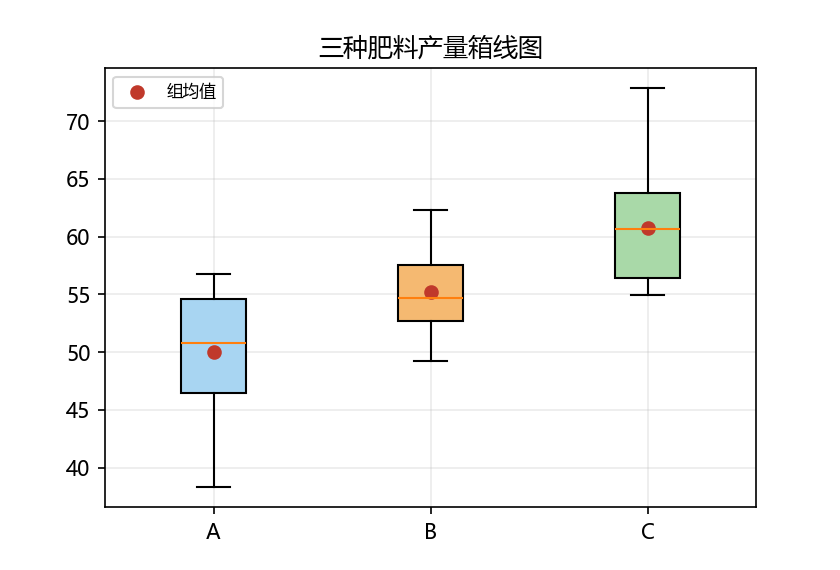
\includegraphics[keepaspectratio,alt={三种肥料的产量箱线图}]{figures/07-statsmodels/case1_fertilizer_anova.png}}
\caption{三种肥料的产量箱线图}
\end{figure}

\subsubsection{主要用法 / API}\label{ux4e3bux8981ux7528ux6cd5-api-28}

{\def\LTcaptype{none} % do not increment counter
\begin{longtable}[]{@{}
  >{\raggedright\arraybackslash}p{(\linewidth - 4\tabcolsep) * \real{0.3333}}
  >{\raggedright\arraybackslash}p{(\linewidth - 4\tabcolsep) * \real{0.3333}}
  >{\raggedright\arraybackslash}p{(\linewidth - 4\tabcolsep) * \real{0.3333}}@{}}
\toprule\noalign{}
\begin{minipage}[b]{\linewidth}\raggedright
需求
\end{minipage} & \begin{minipage}[b]{\linewidth}\raggedright
写法
\end{minipage} & \begin{minipage}[b]{\linewidth}\raggedright
说明
\end{minipage} \\
\midrule\noalign{}
\endhead
\bottomrule\noalign{}
\endlastfoot
生成正态随机数 & \texttt{rng.normal(mean,\ std,\ n)} & 模拟每组产量 \\
按组求均值 &
\texttt{df.groupby(\textquotesingle{}fertilizer\textquotesingle{}){[}\textquotesingle{}out\textquotesingle{}{]}.mean()}
& 组间比较第一步 \\
分类变量进公式 &
\texttt{ols(\textquotesingle{}out\ \textasciitilde{}\ C(fertilizer)\textquotesingle{},\ data=df)}
& \texttt{C()} 把类别变哑变量 \\
方差分析表 & \texttt{sm.stats.anova\_lm(model,\ typ=1)} & 输出
df/平方和/F/P \\
取 F / P 值 &
\texttt{anova{[}\textquotesingle{}F\textquotesingle{}{]}.iloc{[}0{]}} /
\texttt{anova{[}\textquotesingle{}PR(\textgreater{}F)\textquotesingle{}{]}.iloc{[}0{]}}
& 用 \texttt{.iloc{[}0{]}} 避免位置弃用警告 \\
画箱线图 & \texttt{plt.boxplot({[}a,\ b,\ c{]},\ tick\_labels=...)} &
直观展示组分布与均值 \\
\end{longtable}
}

\subsubsection{常见错误}\label{ux5e38ux89c1ux9519ux8bef-28}

\begin{enumerate}
\def\labelenumi{\arabic{enumi}.}
\tightlist
\item
  误把``组均值看起来不同''当成``显著不同''：还要看组内波动（\texttt{SS\_within}）够不够小；组内波动大时，均值差异可能不显著。
\item
  公式里直接写
  \texttt{ols(\textquotesingle{}out\ \textasciitilde{}\ fertilizer\textquotesingle{},\ ...)}
  而不加 \texttt{C()}：字符串列会被 patsy 当连续变量或报错。
\item
  直接用
  \texttt{anova{[}\textquotesingle{}F\textquotesingle{}{]}{[}0{]}}
  取第一行：新版 pandas 可能给出``按位置取数''的 FutureWarning，应改用
  \texttt{.iloc{[}0{]}}。
\item
  忘记在绘图前
  \texttt{os.makedirs(\textquotesingle{}images\textquotesingle{},\ exist\_ok=True)}：首次没有
  \texttt{figures/07-statsmodels/} 目录时 \texttt{savefig} 会报错。
\end{enumerate}

\subsubsection{拓展 / 跟练}\label{ux62d3ux5c55-ux8ddfux7ec3-16}

\begin{enumerate}
\def\labelenumi{\arabic{enumi}.}
\tightlist
\item
  把 \texttt{n} 改成 30，观察 F 与 P
  值如何变化；把种子改成别的值，多次运行看结论是否稳定。
\item
  用 \texttt{scipy.stats.f\_oneway(a,\ b,\ c)} 直接计算，和
  \texttt{anova\_lm} 的 F/P 对比是否一致。
\item
  给数据再加一个``对照''组（不施肥、均值 45），看 4 组 ANOVA 结论。
\item
  用 \texttt{statsmodels.stats.multicomp.pairwise\_tukeyhsd} 做 Tukey
  事后两两比较，找出哪两组差异显著。
\end{enumerate}

\begin{center}\rule{0.5\linewidth}{0.5pt}\end{center}

\subsection{2 线性回归（OLS）}\label{ux7ebfux6027ux56deux5f52ols}

\subsubsection{2.1
数组接口：sm.OLS}\label{ux6570ux7ec4ux63a5ux53e3sm.ols}

数组接口要求手动加截距列（add\_constant），适合已用 NumPy
准备数据的场景。

\begin{Shaded}
\begin{Highlighting}[]
\ImportTok{import}\NormalTok{ numpy }\ImportTok{as}\NormalTok{ np}
\ImportTok{import}\NormalTok{ statsmodels.api }\ImportTok{as}\NormalTok{ sm}

\NormalTok{rng }\OperatorTok{=}\NormalTok{ np.random.default\_rng(}\DecValTok{0}\NormalTok{)}
\NormalTok{x }\OperatorTok{=}\NormalTok{ np.linspace(}\DecValTok{0}\NormalTok{, }\DecValTok{10}\NormalTok{, }\DecValTok{50}\NormalTok{)}
\NormalTok{y }\OperatorTok{=} \DecValTok{2}\OperatorTok{*}\NormalTok{x }\OperatorTok{+} \DecValTok{1} \OperatorTok{+}\NormalTok{ rng.normal(}\DecValTok{0}\NormalTok{, }\DecValTok{1}\NormalTok{, size}\OperatorTok{=}\BuiltInTok{len}\NormalTok{(x))}

\NormalTok{X }\OperatorTok{=}\NormalTok{ sm.add\_constant(x.reshape(}\OperatorTok{{-}}\DecValTok{1}\NormalTok{, }\DecValTok{1}\NormalTok{))}
\NormalTok{model }\OperatorTok{=}\NormalTok{ sm.OLS(y, X).fit()}
\BuiltInTok{print}\NormalTok{(}\StringTok{"params:"}\NormalTok{, model.params)}
\BuiltInTok{print}\NormalTok{(}\StringTok{"R²:"}\NormalTok{, model.rsquared)}
\BuiltInTok{print}\NormalTok{(model.summary())}
\end{Highlighting}
\end{Shaded}

运行结果（Date/Time 随运行时间变化）：

\begin{Shaded}
\begin{Highlighting}[]
\NormalTok{params: [0.54884546 2.1160302 ]}
\NormalTok{R²: 0.9819621414581136}

\NormalTok{                            OLS Regression Results}
\NormalTok{==============================================================================}
\NormalTok{Dep. Variable:                      y   R{-}squared:                       0.982}
\NormalTok{Model:                            OLS   Adj. R{-}squared:                  0.982}
\NormalTok{Method:                 Least Squares   F{-}statistic:                     2613.}
\NormalTok{Date:                Wed, 26 Aug 2026   Prob (F{-}statistic):           1.63e{-}43}
\NormalTok{Time:                        14:08:23   Log{-}Likelihood:                {-}62.504}
\NormalTok{No. Observations:                  50   AIC:                             129.0}
\NormalTok{Df Residuals:                      48   BIC:                             132.8}
\NormalTok{Df Model:                           1}
\NormalTok{Covariance Type:            nonrobust}
\NormalTok{==============================================================================}
\NormalTok{                 coef    std err          t      P\textgreater{}|t|      [0.025      0.975]}
\NormalTok{{-}{-}{-}{-}{-}{-}{-}{-}{-}{-}{-}{-}{-}{-}{-}{-}{-}{-}{-}{-}{-}{-}{-}{-}{-}{-}{-}{-}{-}{-}{-}{-}{-}{-}{-}{-}{-}{-}{-}{-}{-}{-}{-}{-}{-}{-}{-}{-}{-}{-}{-}{-}{-}{-}{-}{-}{-}{-}{-}{-}{-}{-}{-}{-}{-}{-}{-}{-}{-}{-}{-}{-}{-}{-}{-}{-}{-}{-}}
\NormalTok{const          0.5488      0.240      2.285      0.027       0.066       1.032}
\NormalTok{x1             2.1160      0.041     51.118      0.000       2.033       2.199}
\NormalTok{==============================================================================}
\NormalTok{Omnibus:                        0.794   Durbin{-}Watson:                   1.565}
\NormalTok{Prob(Omnibus):                  0.672   Jarque{-}Bera (JB):                0.889}
\NormalTok{Skew:                          {-}0.229   Prob(JB):                        0.641}
\NormalTok{Kurtosis:                       2.533   Cond. No.                         11.7}
\NormalTok{==============================================================================}

\NormalTok{Notes:}
\NormalTok{[1] Standard Errors assume that the covariance matrix of the errors is correctly specified.}
\end{Highlighting}
\end{Shaded}

\begin{figure}
\centering
\pandocbounded{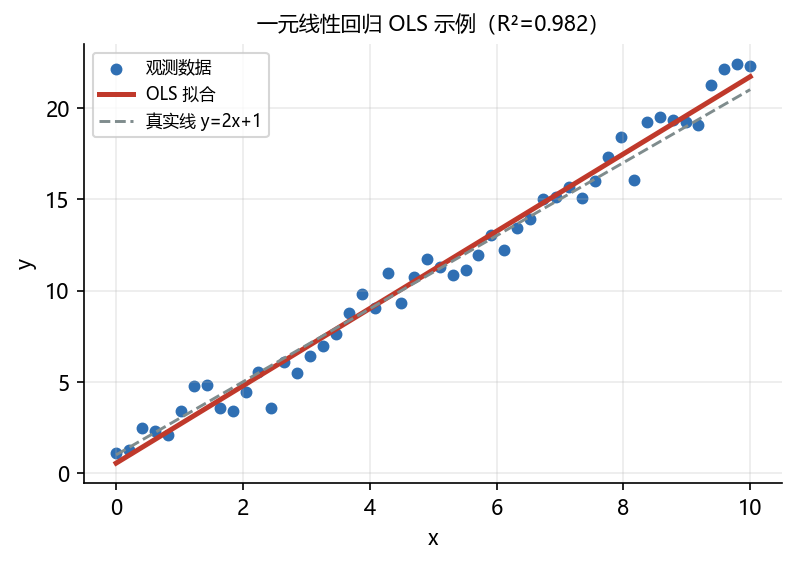
\includegraphics[keepaspectratio,alt={OLS 拟合示意}]{figures/07-statsmodels/regression_ols.png}}
\caption{OLS 拟合示意}
\end{figure}

\textbf{解读要点}：

\begin{itemize}
\tightlist
\item
  截距 const ≈ 0.549，斜率 x1 ≈ 2.116，接近真实值 \((1, 2)\)；
\item
  R²=0.982：模型解释了约 98.2\% 的方差；Adj. R² 对自变量个数做了惩罚；
\item
  F-statistic 与 Prob(F) 是整体显著性检验；Prob(F) ≈
  1.6e-43，模型整体显著；
\item
  每个系数的 P\textgreater\textbar t\textbar{} 是该变量是否显著（0.05
  为常用阈值）；
\item
  {[}0.025, 0.975{]} 是 95\% 置信区间。
\end{itemize}

\subsubsection{2.2 公式接口：ols}\label{ux516cux5f0fux63a5ux53e3ols}

把数据放进 DataFrame，即可用公式写模型：

\begin{Shaded}
\begin{Highlighting}[]
\ImportTok{import}\NormalTok{ pandas }\ImportTok{as}\NormalTok{ pd}
\ImportTok{from}\NormalTok{ statsmodels.formula.api }\ImportTok{import}\NormalTok{ ols}

\NormalTok{x }\OperatorTok{=}\NormalTok{ np.linspace(}\DecValTok{0}\NormalTok{, }\DecValTok{10}\NormalTok{, }\DecValTok{50}\NormalTok{)}
\NormalTok{y }\OperatorTok{=} \DecValTok{2}\OperatorTok{*}\NormalTok{x }\OperatorTok{+} \DecValTok{1} \OperatorTok{+}\NormalTok{ rng.normal(}\DecValTok{0}\NormalTok{, }\DecValTok{1}\NormalTok{, size}\OperatorTok{=}\BuiltInTok{len}\NormalTok{(x))}
\NormalTok{df2 }\OperatorTok{=}\NormalTok{ pd.DataFrame(\{}\StringTok{\textquotesingle{}x\textquotesingle{}}\NormalTok{: x, }\StringTok{\textquotesingle{}y\textquotesingle{}}\NormalTok{: y\})}
\NormalTok{fm }\OperatorTok{=}\NormalTok{ ols(}\StringTok{\textquotesingle{}y \textasciitilde{} x\textquotesingle{}}\NormalTok{, data}\OperatorTok{=}\NormalTok{df2).fit()}
\BuiltInTok{print}\NormalTok{(fm.params)}
\BuiltInTok{print}\NormalTok{(fm.summary())}
\end{Highlighting}
\end{Shaded}

运行结果：

\begin{Shaded}
\begin{Highlighting}[]
\NormalTok{Intercept    0.548845}
\NormalTok{x            2.116030}
\NormalTok{dtype: float64}
\end{Highlighting}
\end{Shaded}

可见公式接口默认加截距（Intercept），且列名直接用 x。其余统计量与 2.1
完全一致。

\subsubsection{2.3 多元回归}\label{ux591aux5143ux56deux5f52}

\begin{Shaded}
\begin{Highlighting}[]
\NormalTok{rng }\OperatorTok{=}\NormalTok{ np.random.default\_rng(}\DecValTok{2}\NormalTok{)}
\NormalTok{x1 }\OperatorTok{=}\NormalTok{ rng.uniform(}\DecValTok{0}\NormalTok{, }\DecValTok{10}\NormalTok{, }\DecValTok{60}\NormalTok{)}
\NormalTok{x2 }\OperatorTok{=}\NormalTok{ rng.uniform(}\OperatorTok{{-}}\DecValTok{3}\NormalTok{, }\DecValTok{3}\NormalTok{, }\DecValTok{60}\NormalTok{)}
\NormalTok{y2 }\OperatorTok{=} \DecValTok{1} \OperatorTok{+} \DecValTok{2}\OperatorTok{*}\NormalTok{x1 }\OperatorTok{{-}} \DecValTok{3}\OperatorTok{*}\NormalTok{x2 }\OperatorTok{+}\NormalTok{ rng.normal(}\DecValTok{0}\NormalTok{, }\DecValTok{1}\NormalTok{, }\DecValTok{60}\NormalTok{)}
\NormalTok{dm }\OperatorTok{=}\NormalTok{ pd.DataFrame(\{}\StringTok{\textquotesingle{}x1\textquotesingle{}}\NormalTok{: x1, }\StringTok{\textquotesingle{}x2\textquotesingle{}}\NormalTok{: x2, }\StringTok{\textquotesingle{}y\textquotesingle{}}\NormalTok{: y2\})}
\NormalTok{mul }\OperatorTok{=}\NormalTok{ ols(}\StringTok{\textquotesingle{}y \textasciitilde{} x1 + x2\textquotesingle{}}\NormalTok{, data}\OperatorTok{=}\NormalTok{dm).fit()}
\BuiltInTok{print}\NormalTok{(mul.params)}
\BuiltInTok{print}\NormalTok{(mul.pvalues)}
\BuiltInTok{print}\NormalTok{(}\StringTok{"R² ="}\NormalTok{, mul.rsquared)}
\end{Highlighting}
\end{Shaded}

运行结果：

\begin{Shaded}
\begin{Highlighting}[]
\NormalTok{Intercept    0.938724}
\NormalTok{x1           1.994930}
\NormalTok{x2          {-}3.056829}
\NormalTok{dtype: float64}
\NormalTok{Intercept    4.204720e{-}04}
\NormalTok{x1           3.299329e{-}47}
\NormalTok{x2           4.863608e{-}49}
\NormalTok{dtype: float64}
\NormalTok{R² = 0.9867366706540099}
\end{Highlighting}
\end{Shaded}

说明：两个自变量的 P 值都远小于 0.05，均显著；系数接近真实值
\((2, -3)\)。

\subsubsection{2.4
公式写法小结}\label{ux516cux5f0fux5199ux6cd5ux5c0fux7ed3}

{\def\LTcaptype{none} % do not increment counter
\begin{longtable}[]{@{}ll@{}}
\toprule\noalign{}
写法 & 含义 \\
\midrule\noalign{}
\endhead
\bottomrule\noalign{}
\endlastfoot
y \textasciitilde{} x & 一元线性 \\
y \textasciitilde{} x1 + x2 & 多元线性（可加性） \\
y \textasciitilde{} C(group) & 把 group 当分类变量（用于 ANOVA） \\
y \textasciitilde{} x1 * x2 & 主效应 + 交互项 \\
y \textasciitilde{} x1 + I(x1**2) & 添加二次项 \\
\end{longtable}
}

\subsection{案例卡 2：OLS 多元回归------用公式接口解读系数与 p
值}\label{ux6848ux4f8bux5361-2ols-ux591aux5143ux56deux5f52ux7528ux516cux5f0fux63a5ux53e3ux89e3ux8bfbux7cfbux6570ux4e0e-p-ux503c}

\subsubsection{目标}\label{ux76eeux6807-28}

造一份``房子面积（平方米）、房龄（年）→
房价（万元）''的模拟数据，用\textbf{公式接口}
\texttt{ols(\textquotesingle{}price\ \textasciitilde{}\ area\ +\ age\textquotesingle{},\ data=df)}
一次估计两个自变量。我们重点关注每个系数的\textbf{大小、符号、p 值、95\%
置信区间}，并说明``面积每大一平米、房龄每多一年，房价平均怎么变''。

\subsubsection{代码}\label{ux4ee3ux7801-29}

\begin{Shaded}
\begin{Highlighting}[]
\ImportTok{import}\NormalTok{ numpy }\ImportTok{as}\NormalTok{ np}
\ImportTok{import}\NormalTok{ pandas }\ImportTok{as}\NormalTok{ pd}
\ImportTok{from}\NormalTok{ statsmodels.formula.api }\ImportTok{import}\NormalTok{ ols}
\ImportTok{import}\NormalTok{ matplotlib.pyplot }\ImportTok{as}\NormalTok{ plt}
\ImportTok{import}\NormalTok{ os}

\NormalTok{plt.rcParams[}\StringTok{\textquotesingle{}font.sans{-}serif\textquotesingle{}}\NormalTok{] }\OperatorTok{=}\NormalTok{ [}\StringTok{\textquotesingle{}Microsoft YaHei\textquotesingle{}}\NormalTok{, }\StringTok{\textquotesingle{}SimHei\textquotesingle{}}\NormalTok{, }\StringTok{\textquotesingle{}DejaVu Sans\textquotesingle{}}\NormalTok{]}
\NormalTok{plt.rcParams[}\StringTok{\textquotesingle{}axes.unicode\_minus\textquotesingle{}}\NormalTok{] }\OperatorTok{=} \VariableTok{False}
\NormalTok{np.set\_printoptions(precision}\OperatorTok{=}\DecValTok{4}\NormalTok{, suppress}\OperatorTok{=}\VariableTok{True}\NormalTok{)}
\NormalTok{pd.set\_option(}\StringTok{\textquotesingle{}display.width\textquotesingle{}}\NormalTok{, }\DecValTok{100}\NormalTok{)}

\NormalTok{rng }\OperatorTok{=}\NormalTok{ np.random.default\_rng(}\DecValTok{3}\NormalTok{)}
\NormalTok{n }\OperatorTok{=} \DecValTok{40}
\NormalTok{area }\OperatorTok{=}\NormalTok{ rng.uniform(}\DecValTok{30}\NormalTok{, }\DecValTok{120}\NormalTok{, n)    }\CommentTok{\# 面积：30\textasciitilde{}120 平米}
\NormalTok{age }\OperatorTok{=}\NormalTok{ rng.uniform(}\DecValTok{0}\NormalTok{, }\DecValTok{30}\NormalTok{, n)       }\CommentTok{\# 房龄：0\textasciitilde{}30 年}
\NormalTok{price }\OperatorTok{=} \DecValTok{50} \OperatorTok{+} \FloatTok{3.0}\OperatorTok{*}\NormalTok{area }\OperatorTok{{-}} \FloatTok{1.5}\OperatorTok{*}\NormalTok{age }\OperatorTok{+}\NormalTok{ rng.normal(}\DecValTok{0}\NormalTok{, }\DecValTok{8}\NormalTok{, n)  }\CommentTok{\# 真实模型}

\NormalTok{df }\OperatorTok{=}\NormalTok{ pd.DataFrame(\{}\StringTok{\textquotesingle{}area\textquotesingle{}}\NormalTok{: area, }\StringTok{\textquotesingle{}age\textquotesingle{}}\NormalTok{: age, }\StringTok{\textquotesingle{}price\textquotesingle{}}\NormalTok{: price\})}
\NormalTok{model }\OperatorTok{=}\NormalTok{ ols(}\StringTok{\textquotesingle{}price \textasciitilde{} area + age\textquotesingle{}}\NormalTok{, data}\OperatorTok{=}\NormalTok{df).fit()}
\NormalTok{ci }\OperatorTok{=}\NormalTok{ model.conf\_int()}

\BuiltInTok{print}\NormalTok{(}\StringTok{\textquotesingle{}coefficients:\textquotesingle{}}\NormalTok{)}
\ControlFlowTok{for}\NormalTok{ name }\KeywordTok{in}\NormalTok{ [}\StringTok{\textquotesingle{}Intercept\textquotesingle{}}\NormalTok{, }\StringTok{\textquotesingle{}area\textquotesingle{}}\NormalTok{, }\StringTok{\textquotesingle{}age\textquotesingle{}}\NormalTok{]:}
    \BuiltInTok{print}\NormalTok{(}\SpecialStringTok{f"}\SpecialCharTok{\{}\NormalTok{name}\SpecialCharTok{:9s\}}\SpecialStringTok{ coef=}\SpecialCharTok{\{}\NormalTok{model}\SpecialCharTok{.}\NormalTok{params[name]}\SpecialCharTok{:.4f\}}\SpecialStringTok{ p=}\SpecialCharTok{\{}\NormalTok{model}\SpecialCharTok{.}\NormalTok{pvalues[name]}\SpecialCharTok{:.2e\}}\SpecialStringTok{ CI=[}\SpecialCharTok{\{}\NormalTok{ci}\SpecialCharTok{.}\NormalTok{loc[name,}\DecValTok{0}\NormalTok{]}\SpecialCharTok{:.4f\}}\SpecialStringTok{, }\SpecialCharTok{\{}\NormalTok{ci}\SpecialCharTok{.}\NormalTok{loc[name,}\DecValTok{1}\NormalTok{]}\SpecialCharTok{:.4f\}}\SpecialStringTok{]"}\NormalTok{)}
\BuiltInTok{print}\NormalTok{(}\StringTok{\textquotesingle{}R2 =\textquotesingle{}}\NormalTok{, }\BuiltInTok{round}\NormalTok{(model.rsquared, }\DecValTok{4}\NormalTok{))}
\BuiltInTok{print}\NormalTok{(}\StringTok{\textquotesingle{}F =\textquotesingle{}}\NormalTok{, }\BuiltInTok{round}\NormalTok{(model.fvalue, }\DecValTok{3}\NormalTok{), }\StringTok{\textquotesingle{} P(F) = }\SpecialCharTok{\%.3g}\StringTok{\textquotesingle{}} \OperatorTok{\%}\NormalTok{ model.f\_pvalue)}
\BuiltInTok{print}\NormalTok{(}\StringTok{\textquotesingle{}AIC =\textquotesingle{}}\NormalTok{, }\BuiltInTok{round}\NormalTok{(model.aic, }\DecValTok{2}\NormalTok{))}

\NormalTok{os.makedirs(}\StringTok{\textquotesingle{}images\textquotesingle{}}\NormalTok{, exist\_ok}\OperatorTok{=}\VariableTok{True}\NormalTok{)}
\NormalTok{fig, axes }\OperatorTok{=}\NormalTok{ plt.subplots(}\DecValTok{1}\NormalTok{, }\DecValTok{2}\NormalTok{, figsize}\OperatorTok{=}\NormalTok{(}\DecValTok{9}\NormalTok{, }\FloatTok{3.6}\NormalTok{))}
\NormalTok{axes[}\DecValTok{0}\NormalTok{].scatter(model.fittedvalues, df[}\StringTok{\textquotesingle{}price\textquotesingle{}}\NormalTok{], s}\OperatorTok{=}\DecValTok{16}\NormalTok{, color}\OperatorTok{=}\StringTok{\textquotesingle{}\#2f6fb3\textquotesingle{}}\NormalTok{, alpha}\OperatorTok{=}\FloatTok{0.7}\NormalTok{)}
\NormalTok{axes[}\DecValTok{0}\NormalTok{].plot([df[}\StringTok{\textquotesingle{}price\textquotesingle{}}\NormalTok{].}\BuiltInTok{min}\NormalTok{(), df[}\StringTok{\textquotesingle{}price\textquotesingle{}}\NormalTok{].}\BuiltInTok{max}\NormalTok{()], [df[}\StringTok{\textquotesingle{}price\textquotesingle{}}\NormalTok{].}\BuiltInTok{min}\NormalTok{(), df[}\StringTok{\textquotesingle{}price\textquotesingle{}}\NormalTok{].}\BuiltInTok{max}\NormalTok{()], color}\OperatorTok{=}\StringTok{\textquotesingle{}\#c0392b\textquotesingle{}}\NormalTok{, lw}\OperatorTok{=}\FloatTok{1.6}\NormalTok{)}
\NormalTok{axes[}\DecValTok{0}\NormalTok{].set\_xlabel(}\StringTok{\textquotesingle{}拟合值\textquotesingle{}}\NormalTok{)}\OperatorTok{;}\NormalTok{ axes[}\DecValTok{0}\NormalTok{].set\_ylabel(}\StringTok{\textquotesingle{}真实值\textquotesingle{}}\NormalTok{)}\OperatorTok{;}\NormalTok{ axes[}\DecValTok{0}\NormalTok{].set\_title(}\StringTok{\textquotesingle{}拟合值 vs 真实值\textquotesingle{}}\NormalTok{)}
\NormalTok{axes[}\DecValTok{1}\NormalTok{].scatter(model.fittedvalues, model.resid, s}\OperatorTok{=}\DecValTok{16}\NormalTok{, color}\OperatorTok{=}\StringTok{\textquotesingle{}\#3a8f4f\textquotesingle{}}\NormalTok{, alpha}\OperatorTok{=}\FloatTok{0.7}\NormalTok{)}
\NormalTok{axes[}\DecValTok{1}\NormalTok{].axhline(}\DecValTok{0}\NormalTok{, color}\OperatorTok{=}\StringTok{\textquotesingle{}\#c0392b\textquotesingle{}}\NormalTok{, lw}\OperatorTok{=}\FloatTok{1.2}\NormalTok{)}
\NormalTok{axes[}\DecValTok{1}\NormalTok{].set\_xlabel(}\StringTok{\textquotesingle{}拟合值\textquotesingle{}}\NormalTok{)}\OperatorTok{;}\NormalTok{ axes[}\DecValTok{1}\NormalTok{].set\_ylabel(}\StringTok{\textquotesingle{}残差\textquotesingle{}}\NormalTok{)}\OperatorTok{;}\NormalTok{ axes[}\DecValTok{1}\NormalTok{].set\_title(}\StringTok{\textquotesingle{}残差 vs 拟合值\textquotesingle{}}\NormalTok{)}
\ControlFlowTok{for}\NormalTok{ ax }\KeywordTok{in}\NormalTok{ axes:}
\NormalTok{    ax.grid(alpha}\OperatorTok{=}\FloatTok{0.25}\NormalTok{)}
\NormalTok{fig.tight\_layout()}
\NormalTok{fig.savefig(}\StringTok{\textquotesingle{}figures/07{-}statsmodels/case2\_ols\_multi.png\textquotesingle{}}\NormalTok{, dpi}\OperatorTok{=}\DecValTok{150}\NormalTok{)}
\NormalTok{plt.close()}
\BuiltInTok{print}\NormalTok{(}\StringTok{\textquotesingle{}saved figures/07{-}statsmodels/case2\_ols\_multi.png\textquotesingle{}}\NormalTok{)}
\end{Highlighting}
\end{Shaded}

\subsubsection{运行结果（已运行核验）}\label{ux8fd0ux884cux7ed3ux679cux5df2ux8fd0ux884cux6838ux9a8c-27}

\begin{Shaded}
\begin{Highlighting}[]
\NormalTok{coefficients:}
\NormalTok{Intercept coef=50.8786 p=2.16e{-}12 CI=[40.8480, 60.9092]}
\NormalTok{area      coef=2.9799 p=1.59e{-}36 CI=[2.8662, 3.0937]}
\NormalTok{age       coef={-}1.4557 p=8.11e{-}11 CI=[{-}1.7844, {-}1.1269]}
\NormalTok{R2 = 0.9872}
\NormalTok{F = 1425.282  P(F) = 9.82e{-}36}
\NormalTok{AIC = 290.09}
\NormalTok{saved figures/07{-}statsmodels/case2\_ols\_multi.png}
\end{Highlighting}
\end{Shaded}

\subsubsection{讲解}\label{ux8bb2ux89e3-27}

\textbf{一句话解释}：房价 ≈ 一个``起步价'' + 每平米单价 × 面积 −
每年折旧 × 房龄；\texttt{coef} 就是这些单价，\texttt{p}
告诉你``这个单价是不是真的、会不会只是噪声''。

\begin{enumerate}
\def\labelenumi{\arabic{enumi}.}
\tightlist
\item
  \texttt{area\ =\ rng.uniform(30,\ 120,\ n)}：生成 40
  套房子的面积；\texttt{age} 类似。\texttt{price} 用真实系数
  \texttt{(50,\ 3,\ -1.5)}
  再加噪声构造，这样我们能``对着答案''检验模型。
\item
  \texttt{ols(\textquotesingle{}price\ \textasciitilde{}\ area\ +\ age\textquotesingle{},\ data=df)}：公式接口自动加截距（\texttt{Intercept}），并同时放进
  \texttt{area} 与 \texttt{age} 两个自变量。
\item
  \texttt{model.params}：截距 ≈50.88（接近真实 50），\texttt{area}
  ≈2.98（接近真实 3），\texttt{age} ≈−1.46（接近真实
  −1.5）。系数就是``在控制另一个变量后，该变量每改变 1
  单位，因变量的平均变化''。
\item
  \texttt{model.pvalues}：三个 p 值都远小于
  0.05，说明截距、面积、房龄都\textbf{统计显著}；房龄系数为负也符合直觉（房子越旧越便宜）。
\item
  \texttt{model.conf\_int()}：给出 95\% 置信区间。\texttt{area} 的区间
  \texttt{{[}2.87,\ 3.09{]}} 不包含
  0，说明面积效应显著为正；\texttt{age} 区间
  \texttt{{[}-1.78,\ -1.13{]}} 不包含 0，说明房龄效应显著为负。
\item
  \texttt{R2=0.9872}：面积+房龄解释了约 98.7\% 的房价变动；\texttt{F} 与
  \texttt{p(F)} 说明模型整体显著。\texttt{AIC} 可用于与其它模型比较。
\end{enumerate}

\begin{figure}
\centering
\pandocbounded{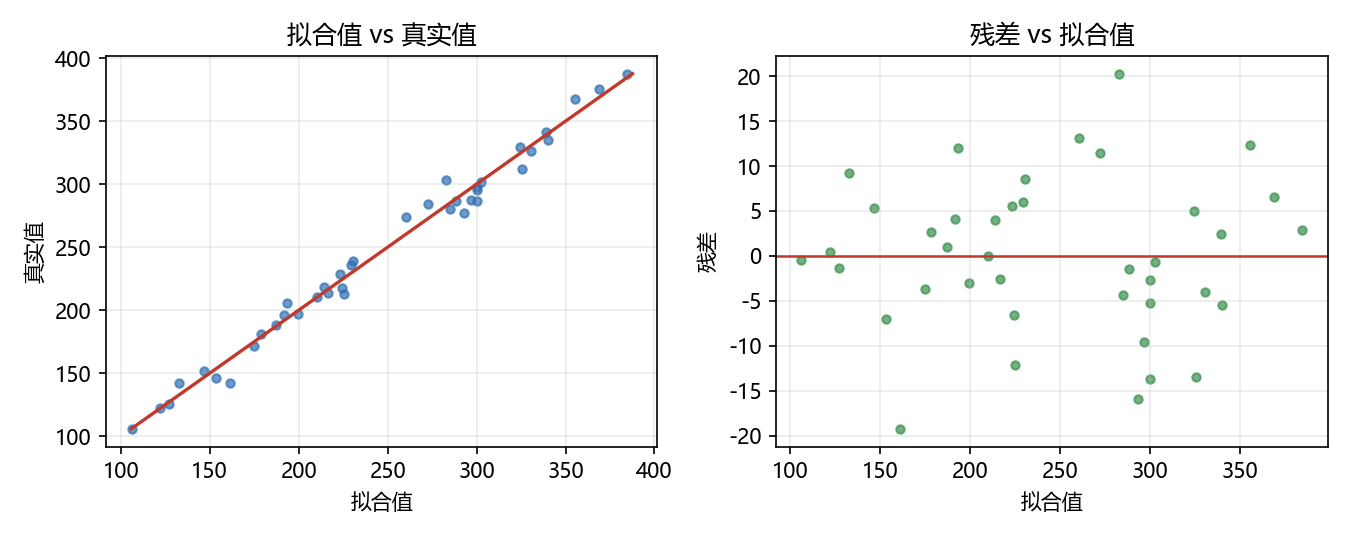
\includegraphics[keepaspectratio,alt={拟合值 vs 真实值 与 残差图}]{figures/07-statsmodels/case2_ols_multi.png}}
\caption{拟合值 vs 真实值 与 残差图}
\end{figure}

\subsubsection{主要用法 / API}\label{ux4e3bux8981ux7528ux6cd5-api-29}

{\def\LTcaptype{none} % do not increment counter
\begin{longtable}[]{@{}
  >{\raggedright\arraybackslash}p{(\linewidth - 4\tabcolsep) * \real{0.3333}}
  >{\raggedright\arraybackslash}p{(\linewidth - 4\tabcolsep) * \real{0.3333}}
  >{\raggedright\arraybackslash}p{(\linewidth - 4\tabcolsep) * \real{0.3333}}@{}}
\toprule\noalign{}
\begin{minipage}[b]{\linewidth}\raggedright
需求
\end{minipage} & \begin{minipage}[b]{\linewidth}\raggedright
写法
\end{minipage} & \begin{minipage}[b]{\linewidth}\raggedright
说明
\end{minipage} \\
\midrule\noalign{}
\endhead
\bottomrule\noalign{}
\endlastfoot
多元回归 &
\texttt{ols(\textquotesingle{}price\ \textasciitilde{}\ area\ +\ age\textquotesingle{},\ data=df)}
& 公式接口，自动加截距 \\
系数 & \texttt{model.params} & 每个变量的边际效应 \\
p 值 & \texttt{model.pvalues} & \textless0.05 视为显著 \\
置信区间 & \texttt{model.conf\_int()} & 95\% CI，不含 0 一般显著 \\
拟合优度 & \texttt{model.rsquared} / \texttt{model.rsquared\_adj} &
解释比例 / 调整后 \\
整体显著性 & \texttt{model.fvalue} / \texttt{model.f\_pvalue} &
所有系数联合是否为 0 \\
信息准则 & \texttt{model.aic} & 越小越好，用于模型选择 \\
\end{longtable}
}

\subsubsection{常见错误}\label{ux5e38ux89c1ux9519ux8bef-29}

\begin{enumerate}
\def\labelenumi{\arabic{enumi}.}
\tightlist
\item
  只打印 \texttt{model.summary()}
  而不使用关键字段：跨版本摘要边缘（空格、分隔线、\texttt{+/-}
  号）不稳定，教学时建议用
  \texttt{params}/\texttt{pvalues}/\texttt{conf\_int} 打印固定字段。
\item
  忘记 \texttt{add\_constant}
  但用了数组接口：公式接口自动加截距，数组接口却要手动加。
\item
  把 \texttt{p=0.0} 直接打印当``无意义''：应使用 \texttt{\%.2e} 或
  \texttt{\%.3g} 科学计数法，避免显示成 0。
\item
  用 \texttt{round(model.pvalues,\ 4)} 输出时 p 值太小被四舍五入成
  0.0000，看不出数量级。
\end{enumerate}

\subsubsection{拓展 / 跟练}\label{ux62d3ux5c55-ux8ddfux7ec3-17}

\begin{enumerate}
\def\labelenumi{\arabic{enumi}.}
\tightlist
\item
  在公式里加交互项
  \texttt{ols(\textquotesingle{}price\ \textasciitilde{}\ area\ +\ age\ +\ area:age\textquotesingle{},\ data=df)}，看交互项是否显著。
\item
  把 \texttt{age} 换成``新房/二手''分类变量
  \texttt{C(new\_house)}，对比系数含义变化。
\item
  用数组接口
  \texttt{sm.OLS(df{[}\textquotesingle{}price\textquotesingle{}{]},\ sm.add\_constant(df{[}{[}\textquotesingle{}area\textquotesingle{},\textquotesingle{}age\textquotesingle{}{]}{]}))}
  重跑，确认系数一致。
\item
  计算各自变量的标准化系数（\texttt{z-score}
  后回归），比较``谁的影响更大''。
\end{enumerate}

\begin{center}\rule{0.5\linewidth}{0.5pt}\end{center}

\subsection{3 回归诊断：残差 QQ 图与 JB
统计量}\label{ux56deux5f52ux8bcaux65adux6b8bux5dee-qq-ux56feux4e0e-jb-ux7edfux8ba1ux91cf}

\subsubsection{3.1 为什么诊断}\label{ux4e3aux4ec0ux4e48ux8bcaux65ad}

OLS 的统计推断（t/F/P
值）依赖于\textbf{误差项独立同分布、同方差、近似正态}。诊断残差是否偏离这些假设，能及时发现模型设定问题。

\begin{Shaded}
\begin{Highlighting}[]
\ImportTok{import}\NormalTok{ matplotlib.pyplot }\ImportTok{as}\NormalTok{ plt}
\NormalTok{rng }\OperatorTok{=}\NormalTok{ np.random.default\_rng(}\DecValTok{0}\NormalTok{)}
\NormalTok{xd }\OperatorTok{=}\NormalTok{ np.linspace(}\DecValTok{0}\NormalTok{, }\DecValTok{10}\NormalTok{, }\DecValTok{50}\NormalTok{)}
\NormalTok{yd }\OperatorTok{=} \DecValTok{3}\OperatorTok{*}\NormalTok{xd }\OperatorTok{+} \DecValTok{2} \OperatorTok{+}\NormalTok{ rng.normal(}\DecValTok{0}\NormalTok{, }\DecValTok{1}\NormalTok{, }\DecValTok{50}\NormalTok{)}
\NormalTok{Xd }\OperatorTok{=}\NormalTok{ sm.add\_constant(xd.reshape(}\OperatorTok{{-}}\DecValTok{1}\NormalTok{, }\DecValTok{1}\NormalTok{))}
\NormalTok{olsd }\OperatorTok{=}\NormalTok{ sm.OLS(yd, Xd).fit()}
\NormalTok{sm.qqplot(olsd.resid, line}\OperatorTok{=}\StringTok{\textquotesingle{}45\textquotesingle{}}\NormalTok{)}
\NormalTok{plt.title(}\StringTok{"残差 QQ 图"}\NormalTok{)}
\NormalTok{plt.show()}
\BuiltInTok{print}\NormalTok{(olsd.summary())}
\end{Highlighting}
\end{Shaded}

在模型摘要中可找到：

\begin{Shaded}
\begin{Highlighting}[]
\NormalTok{Prob(Omnibus):                  0.672   Jarque{-}Bera (JB):                0.889}
\NormalTok{Skew:                          {-}0.229   Prob(JB):                        0.641}
\end{Highlighting}
\end{Shaded}

\begin{figure}
\centering
\pandocbounded{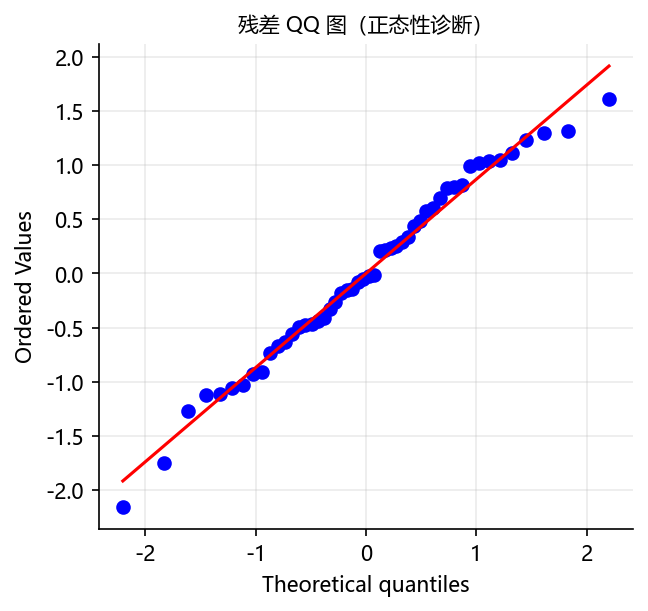
\includegraphics[keepaspectratio,alt={残差 QQ 图}]{figures/07-statsmodels/qq_resid.png}}
\caption{残差 QQ 图}
\end{figure}

\textbf{解读}：

\begin{itemize}
\tightlist
\item
  Jarque-Bera (JB) 检验残差是否为正态分布；Prob(JB)=0.641 \textgreater{}
  0.05，不能拒绝正态假设，说明残差近似正态；
\item
  QQ 图中点应落在 45° 直线附近；本例散点基本沿直线，正态性可接受。
\end{itemize}

\begin{center}\rule{0.5\linewidth}{0.5pt}\end{center}

\subsection{4
广义线性模型（GLM）}\label{ux5e7fux4e49ux7ebfux6027ux6a21ux578bglm}

\subsubsection{4.1 概念}\label{ux6982ux5ff5-1}

当因变量是\textbf{二分类}（成功/失败）、计数或比例时，OLS
不再合适。广义线性模型通过\textbf{链接函数}把线性预测值映射到合理的取值区间，并用指数族分布建模。二分类最常用
Binomial 家族 + Logit 链接（即逻辑回归）：

\[
\text{logit}(p) = \beta_0 + \beta_1 x_1 + \beta_2 x_2,\qquad
p = \frac{1}{1+e^{-(\beta_0+\beta_1 x_1+\beta_2 x_2)}}
\]

\subsubsection{4.2 二分类 Logit
示例}\label{ux4e8cux5206ux7c7b-logit-ux793aux4f8b}

\begin{Shaded}
\begin{Highlighting}[]
\ImportTok{import}\NormalTok{ numpy }\ImportTok{as}\NormalTok{ np}
\ImportTok{import}\NormalTok{ statsmodels.api }\ImportTok{as}\NormalTok{ sm}

\NormalTok{rng }\OperatorTok{=}\NormalTok{ np.random.default\_rng(}\DecValTok{0}\NormalTok{)}
\NormalTok{X\_raw }\OperatorTok{=}\NormalTok{ rng.uniform(}\DecValTok{0}\NormalTok{, }\DecValTok{1}\NormalTok{, (}\DecValTok{200}\NormalTok{, }\DecValTok{2}\NormalTok{))}
\NormalTok{lin }\OperatorTok{=} \FloatTok{0.5} \OperatorTok{+} \FloatTok{1.2}\OperatorTok{*}\NormalTok{X\_raw[:, }\DecValTok{0}\NormalTok{] }\OperatorTok{{-}} \FloatTok{0.8}\OperatorTok{*}\NormalTok{X\_raw[:, }\DecValTok{1}\NormalTok{]}
\NormalTok{p }\OperatorTok{=} \DecValTok{1}\OperatorTok{/}\NormalTok{(}\DecValTok{1}\OperatorTok{+}\NormalTok{np.exp(}\OperatorTok{{-}}\NormalTok{lin))}
\NormalTok{Y }\OperatorTok{=}\NormalTok{ rng.binomial(}\DecValTok{1}\NormalTok{, p)               }\CommentTok{\# 真实概率 p 下的二分类结果}

\NormalTok{X }\OperatorTok{=}\NormalTok{ sm.add\_constant(X\_raw)}
\NormalTok{glm }\OperatorTok{=}\NormalTok{ sm.GLM(Y, X, family}\OperatorTok{=}\NormalTok{sm.families.Binomial()).fit()}
\BuiltInTok{print}\NormalTok{(glm.params)}
\NormalTok{X\_new }\OperatorTok{=}\NormalTok{ sm.add\_constant(np.array([[}\FloatTok{0.2}\NormalTok{, }\FloatTok{0.3}\NormalTok{], [}\FloatTok{0.8}\NormalTok{, }\FloatTok{0.1}\NormalTok{]]))}
\BuiltInTok{print}\NormalTok{(glm.predict(X\_new))}
\end{Highlighting}
\end{Shaded}

运行结果：

\begin{Shaded}
\begin{Highlighting}[]
\NormalTok{params: [ 0.26505589  1.42126589 {-}0.87263185]}
\NormalTok{predict: [0.57138876 0.78831616]}
\end{Highlighting}
\end{Shaded}

\textbf{解读}：

\begin{itemize}
\tightlist
\item
  估计系数接近真实值 \((0.5, 1.2, -0.8)\)，且符号正确（x1 正、x2 负）；
\item
  predict 返回的是\textbf{概率}（经过 Logit
  反变换），两个新样本的成功概率约为 0.57 与 0.79；
\item
  若想得到 0/1 分类，可再对概率设阈值（如 \textgreater0.5 判为 1），见
  04 常见误区。
\end{itemize}

\begin{center}\rule{0.5\linewidth}{0.5pt}\end{center}

\subsection{5
加权最小二乘（WLS）处理异方差}\label{ux52a0ux6743ux6700ux5c0fux4e8cux4e58wlsux5904ux7406ux5f02ux65b9ux5dee}

当误差方差随自变量变化（异方差）时，OLS
虽无偏但效率低（标准误不准）。WLS 用权重 \(w_i\)
加权残差平方和，对异方差更稳健。

\begin{Shaded}
\begin{Highlighting}[]
\ImportTok{import}\NormalTok{ numpy }\ImportTok{as}\NormalTok{ np}
\ImportTok{import}\NormalTok{ statsmodels.api }\ImportTok{as}\NormalTok{ sm}

\NormalTok{rng }\OperatorTok{=}\NormalTok{ np.random.default\_rng(}\DecValTok{1}\NormalTok{)}
\NormalTok{xw }\OperatorTok{=}\NormalTok{ np.linspace(}\FloatTok{0.1}\NormalTok{, }\DecValTok{10}\NormalTok{, }\DecValTok{200}\NormalTok{)}
\NormalTok{eps }\OperatorTok{=}\NormalTok{ rng.normal(}\DecValTok{0}\NormalTok{, xw)            }\CommentTok{\# 标准差与 x 成正比 {-}\textgreater{} 方差与 x\^{}2 成正比}
\NormalTok{yw }\OperatorTok{=} \DecValTok{3}\OperatorTok{*}\NormalTok{xw }\OperatorTok{+}\NormalTok{ eps}
\NormalTok{Xw }\OperatorTok{=}\NormalTok{ sm.add\_constant(xw.reshape(}\OperatorTok{{-}}\DecValTok{1}\NormalTok{, }\DecValTok{1}\NormalTok{))}

\NormalTok{ols\_w }\OperatorTok{=}\NormalTok{ sm.OLS(yw, Xw).fit()}
\NormalTok{wls\_w }\OperatorTok{=}\NormalTok{ sm.WLS(yw, Xw, weights}\OperatorTok{=}\DecValTok{1}\OperatorTok{/}\NormalTok{np.square(xw)).fit()}
\BuiltInTok{print}\NormalTok{(}\StringTok{"OLS:"}\NormalTok{, np.}\BuiltInTok{round}\NormalTok{(ols\_w.params, }\DecValTok{4}\NormalTok{), }\StringTok{"bse"}\NormalTok{, np.}\BuiltInTok{round}\NormalTok{(ols\_w.bse, }\DecValTok{4}\NormalTok{))}
\BuiltInTok{print}\NormalTok{(}\StringTok{"WLS:"}\NormalTok{, np.}\BuiltInTok{round}\NormalTok{(wls\_w.params, }\DecValTok{4}\NormalTok{), }\StringTok{"bse"}\NormalTok{, np.}\BuiltInTok{round}\NormalTok{(wls\_w.bse, }\DecValTok{4}\NormalTok{))}
\end{Highlighting}
\end{Shaded}

运行结果：

\begin{Shaded}
\begin{Highlighting}[]
\NormalTok{OLS: [{-}0.0422  2.9257] bse [0.833  0.1434]}
\NormalTok{WLS: [ 0.0597  2.8971] bse [0.0641 0.0727]}
\end{Highlighting}
\end{Shaded}

\textbf{解读}：

\begin{itemize}
\tightlist
\item
  两者斜率都接近真实值 3；
\item
  但 WLS 的斜率标准误（0.0727）明显小于
  OLS（0.1434），说明在已知异方差形式（\(\sigma_i \propto x_i\)）时，WLS
  估计更有效。
\end{itemize}

\begin{center}\rule{0.5\linewidth}{0.5pt}\end{center}

\subsection{6
方差分析与回归的统一框架}\label{ux65b9ux5deeux5206ux6790ux4e0eux56deux5f52ux7684ux7edfux4e00ux6846ux67b6}

线性回归与方差分析其实共享同一套\textbf{线性模型 + 最小二乘 + F
检验}逻辑：

\begin{itemize}
\tightlist
\item
  回归用连续/哑变量做\textbf{解释}；ANOVA 用分组哑变量做\textbf{比较}；
\item
  都可以写成 \(y = X\beta + \varepsilon\)，用 ols 拟合；
\item
  都能用 F 检验判断``若干系数同时为 0''的联合显著性。
\end{itemize}

因此，ANOVA
可看成\textbf{只有分类自变量}的线性回归；回归也可看成含连续+分类变量的``广义''ANOVA。这就是为什么要用
ols + anova\_lm 而不是单独的 scipy.stats.f\_oneway 来统一步骤。

\begin{center}\rule{0.5\linewidth}{0.5pt}\end{center}

\subsection{常见误区}\label{ux5e38ux89c1ux8befux533a-20}

\begin{enumerate}
\def\labelenumi{\arabic{enumi}.}
\tightlist
\item
  \textbf{忘记加截距}：数组接口必须 X =
  sm.add\_constant(X)，否则模型强制过原点。
\item
  **用 * 表示``与''\textbf{：公式里 y \textasciitilde{} x1 * x2
  是主效应+交互项，不是数值乘法；要写原生项用 I(x1}2) 且注意加
  I(\ldots)。
\item
  \textbf{分类变量直接进公式}：对字符串列，ols(`y \textasciitilde{}
  group') 会当成连续变量或报错，应写成 C(group)。
\item
  \textbf{用 predict 忘记加常数}：数组接口预测新数据也要
  sm.add\_constant(X\_new)。
\item
  \textbf{把 GLM 的 predict 当分类输出}：默认返回概率，需要阈值才能变
  0/1。
\item
  \textbf{忽略诊断}：只报 R² 不看不残差与显著性检验，容易过拟合/误设。
\end{enumerate}

\subsection{思考题}\label{ux601dux8003ux9898-22}

\begin{enumerate}
\def\labelenumi{\arabic{enumi}.}
\tightlist
\item
  为什么数组接口里 add\_constant
  必须加？如果不加，拟合结果在什么情况下仍``正确''？
\item
  anova\_lm(model, typ=1) 与 typ=3
  在单因素时结果是否相同？在多因素时为何可能不同？
\item
  给定 y \textasciitilde{} x1 + x2，若想加入 x1 与 x2
  的交互，公式应怎么写？系数个数变成几个？
\item
  为什么 GLM 不用 OLS 直接拟合二分类因变量？（提示：概率会越界、异方差）
\end{enumerate}

\subsection{动手练习（详见
lab）}\label{ux52a8ux624bux7ec3ux4e60ux8be6ux89c1-lab-14}

\begin{itemize}
\tightlist
\item
  用 sm.OLS 拟合 y = 1 + 2x 的噪声数据，打印完整 summary()；
\item
  构造三个组，画出箱线图并做单因素方差分析；
\item
  用公式 API 拟合 y \textasciitilde{} x1 + x2，说明各系数显著性；
\item
  用 GLM(Binomial) 拟合二分类数据，并在不同阈值下计算准确率与 F1。
\end{itemize}

\subsection{延伸阅读}\label{ux5ef6ux4f38ux9605ux8bfb-31}

\begin{itemize}
\tightlist
\item
  statsmodels Regressions
  官方：\href{https://www.statsmodels.org/stable/regression.html}{链接}
\item
  statsmodels GLM
  官方：\href{https://www.statsmodels.org/stable/glm.html}{链接}
\item
  残差诊断（Statsmodels
  图示）：\href{https://www.statsmodels.org/stable/examples/index.html\#regression}{链接}
\end{itemize}

\section{02 时间序列预测}\label{ux65f6ux95f4ux5e8fux5217ux9884ux6d4b}

\begin{quote}
本节对应原版 7.2 的内容，并增补目标、平稳性检验实操与思考题。
配套图：figures/07-statsmodels/decompose\_daily.png、figures/07-statsmodels/arima\_forecast.png（由
build/make\_chap7\_figures.py 生成）。
\end{quote}

\subsection{本节目标}\label{ux672cux8282ux76eeux6807-27}

\begin{itemize}
\tightlist
\item
  会用 seasonal\_decompose 把时间序列分解为趋势、季节、残差；
\item
  会用 adfuller 做单位根检验，判断序列是否平稳；
\item
  会用 ARIMA 拟合时间序列并给出未来预测；
\item
  会从 ACF/PACF 或网格搜索选择 (p, d, q) 阶数；
\item
  能画分解图与预测图，并解读结果。
\end{itemize}

\subsection{先修}\label{ux5148ux4fee-20}

\begin{itemize}
\tightlist
\item
  Pandas 时间序列索引（date\_range、Series）；本章第 01
  节的回归/统计基础。
\item
  已安装 statsmodels（见章 README）。
\end{itemize}

\subsection{官方文档/参考入口}\label{ux5b98ux65b9ux6587ux6863ux53c2ux8003ux5165ux53e3-6}

{\def\LTcaptype{none} % do not increment counter
\begin{longtable}[]{@{}
  >{\raggedright\arraybackslash}p{(\linewidth - 4\tabcolsep) * \real{0.3333}}
  >{\raggedright\arraybackslash}p{(\linewidth - 4\tabcolsep) * \real{0.3333}}
  >{\raggedright\arraybackslash}p{(\linewidth - 4\tabcolsep) * \real{0.3333}}@{}}
\toprule\noalign{}
\begin{minipage}[b]{\linewidth}\raggedright
内容
\end{minipage} & \begin{minipage}[b]{\linewidth}\raggedright
链接
\end{minipage} & \begin{minipage}[b]{\linewidth}\raggedright
说明
\end{minipage} \\
\midrule\noalign{}
\endhead
\bottomrule\noalign{}
\endlastfoot
seasonal\_decompose &
\href{https://www.statsmodels.org/stable/generated/statsmodels.tsa.seasonal.seasonal_decompose.html}{链接}
& 时间序列分解 \\
adfuller &
\href{https://www.statsmodels.org/stable/generated/statsmodels.tsa.stattools.adfuller.html}{链接}
& ADF 单位根检验 \\
ARIMA &
\href{https://www.statsmodels.org/stable/generated/statsmodels.tsa.arima.model.ARIMA.html}{链接}
& ARIMA 模型 \\
时间序列官方教程 &
\href{https://www.statsmodels.org/stable/tsa.html}{链接} &
时间序列总览 \\
\end{longtable}
}

\begin{center}\rule{0.5\linewidth}{0.5pt}\end{center}

\subsection{1
时间序列分解（seasonal\_decompose）}\label{ux65f6ux95f4ux5e8fux5217ux5206ux89e3seasonal_decompose}

\subsubsection{1.1 概念}\label{ux6982ux5ff5-2}

把序列 \(y_t\) 拆成三部分：

\[
y_t = T_t + S_t + R_t \quad(\text{加法模型})
\qquad\text{或}\qquad
y_t = T_t \times S_t \times R_t \quad(\text{乘法模型})
\]

其中 \(T_t\) 是\textbf{趋势}、\(S_t\) 是\textbf{季节}、\(R_t\)
是\textbf{残差}。加法模型适合波动幅度不随水平变化的序列；乘法模型适合幅度随水平增长的序列。

\subsubsection{1.2 日数据（周期=7
天）}\label{ux65e5ux6570ux636eux5468ux671f7-ux5929}

构造 180 天日序列：线性趋势 + 周季节性（正弦，周期 7）+ 噪声。

\begin{Shaded}
\begin{Highlighting}[]
\ImportTok{import}\NormalTok{ numpy }\ImportTok{as}\NormalTok{ np}
\ImportTok{import}\NormalTok{ pandas }\ImportTok{as}\NormalTok{ pd}
\ImportTok{import}\NormalTok{ statsmodels.api }\ImportTok{as}\NormalTok{ sm}
\ImportTok{import}\NormalTok{ matplotlib.pyplot }\ImportTok{as}\NormalTok{ plt}
\ImportTok{from}\NormalTok{ statsmodels.tsa.seasonal }\ImportTok{import}\NormalTok{ seasonal\_decompose}

\NormalTok{plt.rcParams[}\StringTok{\textquotesingle{}font.sans{-}serif\textquotesingle{}}\NormalTok{] }\OperatorTok{=}\NormalTok{ [}\StringTok{\textquotesingle{}Microsoft YaHei\textquotesingle{}}\NormalTok{, }\StringTok{\textquotesingle{}SimHei\textquotesingle{}}\NormalTok{, }\StringTok{\textquotesingle{}DejaVu Sans\textquotesingle{}}\NormalTok{]}
\NormalTok{plt.rcParams[}\StringTok{\textquotesingle{}axes.unicode\_minus\textquotesingle{}}\NormalTok{] }\OperatorTok{=} \VariableTok{False}

\NormalTok{rng }\OperatorTok{=}\NormalTok{ np.random.default\_rng(}\DecValTok{0}\NormalTok{)}
\NormalTok{idx }\OperatorTok{=}\NormalTok{ pd.date\_range(}\StringTok{\textquotesingle{}2022{-}01{-}01\textquotesingle{}}\NormalTok{, periods}\OperatorTok{=}\DecValTok{180}\NormalTok{, freq}\OperatorTok{=}\StringTok{\textquotesingle{}D\textquotesingle{}}\NormalTok{)}
\NormalTok{trend }\OperatorTok{=}\NormalTok{ np.linspace(}\DecValTok{0}\NormalTok{, }\DecValTok{5}\NormalTok{, }\BuiltInTok{len}\NormalTok{(idx))}
\NormalTok{season }\OperatorTok{=} \DecValTok{2}\OperatorTok{*}\NormalTok{np.sin(}\DecValTok{2}\OperatorTok{*}\NormalTok{np.pi}\OperatorTok{*}\NormalTok{np.arange(}\BuiltInTok{len}\NormalTok{(idx))}\OperatorTok{/}\DecValTok{7}\NormalTok{)}
\NormalTok{noise }\OperatorTok{=}\NormalTok{ rng.normal(}\DecValTok{0}\NormalTok{, }\FloatTok{0.5}\NormalTok{, }\BuiltInTok{len}\NormalTok{(idx))}
\NormalTok{s }\OperatorTok{=}\NormalTok{ pd.Series(}\DecValTok{10} \OperatorTok{+}\NormalTok{ trend }\OperatorTok{+}\NormalTok{ season }\OperatorTok{+}\NormalTok{ noise, index}\OperatorTok{=}\NormalTok{idx)}

\NormalTok{result }\OperatorTok{=}\NormalTok{ seasonal\_decompose(s, model}\OperatorTok{=}\StringTok{\textquotesingle{}additive\textquotesingle{}}\NormalTok{, period}\OperatorTok{=}\DecValTok{7}\NormalTok{)}
\BuiltInTok{print}\NormalTok{(}\StringTok{"trend head:"}\NormalTok{, np.}\BuiltInTok{round}\NormalTok{(result.trend.head(}\DecValTok{7}\NormalTok{).values, }\DecValTok{3}\NormalTok{))}
\BuiltInTok{print}\NormalTok{(}\StringTok{"seasonal head:"}\NormalTok{, np.}\BuiltInTok{round}\NormalTok{(result.seasonal.head(}\DecValTok{7}\NormalTok{).values, }\DecValTok{3}\NormalTok{))}
\BuiltInTok{print}\NormalTok{(}\StringTok{"resid describe:"}\NormalTok{, result.resid.describe().}\BuiltInTok{round}\NormalTok{(}\DecValTok{4}\NormalTok{).to\_dict())}
\NormalTok{result.plot()}
\NormalTok{plt.show()}
\end{Highlighting}
\end{Shaded}

运行结果：

\begin{Shaded}
\begin{Highlighting}[]
\NormalTok{trend head: [   nan    nan    nan 10.217 10.304 10.291 10.183]}
\NormalTok{seasonal head: [ 0.08   1.485  2.005  0.898 {-}0.765 {-}2.135 {-}1.567]}
\NormalTok{resid describe: \{\textquotesingle{}count\textquotesingle{}: 174.0, \textquotesingle{}mean\textquotesingle{}: {-}0.0018, \textquotesingle{}std\textquotesingle{}: 0.4279, \textquotesingle{}min\textquotesingle{}: {-}1.3175, \textquotesingle{}25\%\textquotesingle{}: {-}0.3194, \textquotesingle{}50\%\textquotesingle{}: 0.0279, \textquotesingle{}75\%\textquotesingle{}: 0.3018, \textquotesingle{}max\textquotesingle{}: 0.9416\}}
\end{Highlighting}
\end{Shaded}

\begin{figure}
\centering
\pandocbounded{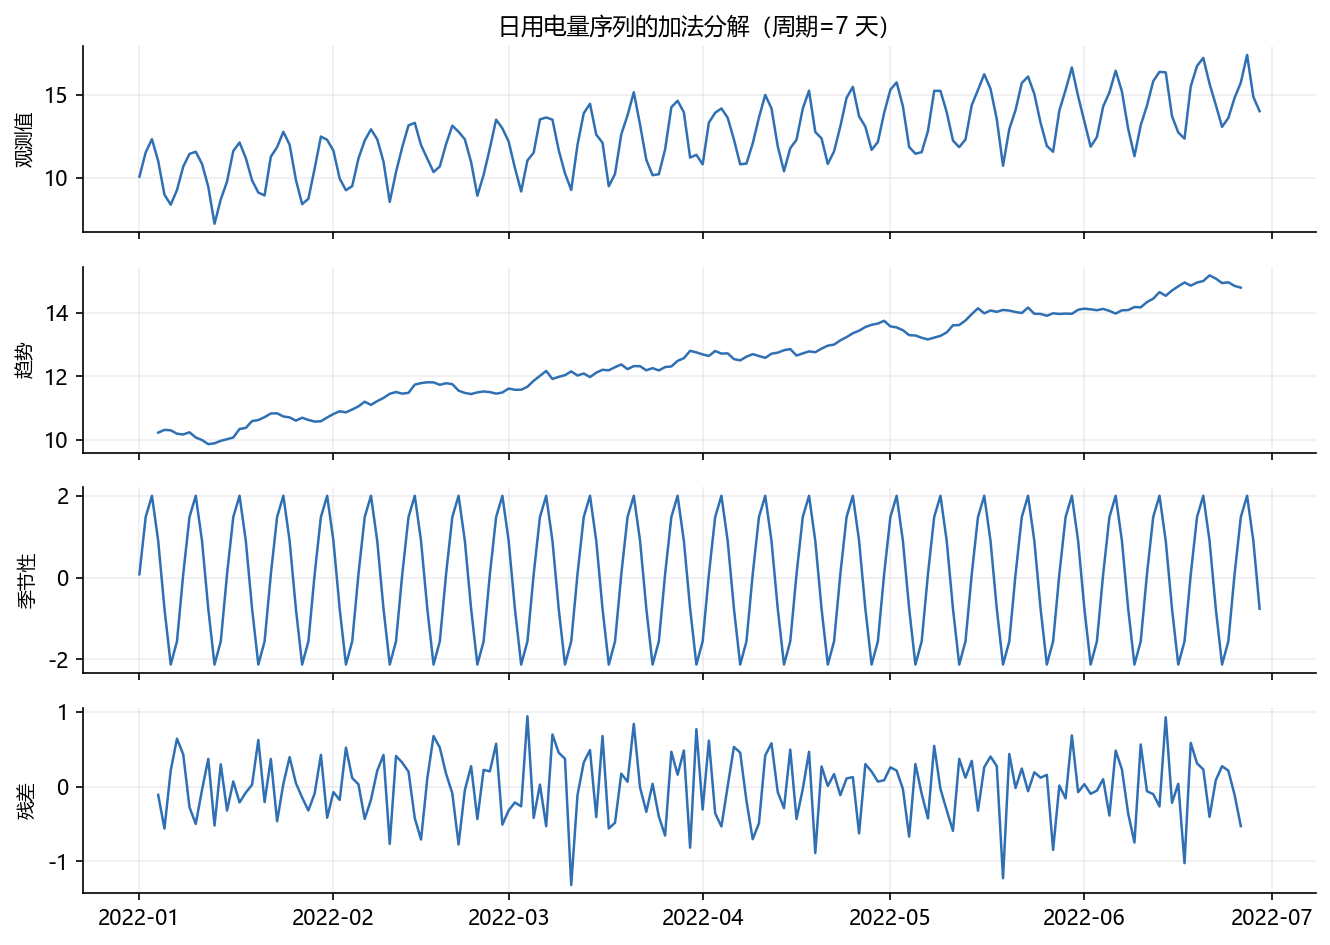
\includegraphics[keepaspectratio,alt={日序列加法分解}]{figures/07-statsmodels/decompose_daily.png}}
\caption{日序列加法分解}
\end{figure}

\textbf{解读}：

\begin{itemize}
\tightlist
\item
  trend 前 3 个是 NaN，因为居中的移动平均在两端没有完整窗口；
\item
  seasonal 在 7 天内正负交替（周一/周末的效应），幅度约 ±2；
\item
  残差均值接近 0、标准差约 0.43，与设定的噪声尺度（0.5）相符。
\end{itemize}

\subsubsection{1.3 月度数据（周期=12
个月）}\label{ux6708ux5ea6ux6570ux636eux5468ux671f12-ux4e2aux6708}

\begin{Shaded}
\begin{Highlighting}[]
\NormalTok{rng }\OperatorTok{=}\NormalTok{ np.random.default\_rng(}\DecValTok{5}\NormalTok{)}
\NormalTok{idxm }\OperatorTok{=}\NormalTok{ pd.date\_range(}\StringTok{\textquotesingle{}2019{-}01{-}01\textquotesingle{}}\NormalTok{, periods}\OperatorTok{=}\DecValTok{36}\NormalTok{, freq}\OperatorTok{=}\StringTok{\textquotesingle{}MS\textquotesingle{}}\NormalTok{)}
\NormalTok{trendm }\OperatorTok{=}\NormalTok{ np.linspace(}\DecValTok{0}\NormalTok{, }\DecValTok{12}\NormalTok{, }\BuiltInTok{len}\NormalTok{(idxm))}
\NormalTok{seasonm }\OperatorTok{=} \DecValTok{3}\OperatorTok{*}\NormalTok{np.sin(}\DecValTok{2}\OperatorTok{*}\NormalTok{np.pi}\OperatorTok{*}\NormalTok{np.arange(}\BuiltInTok{len}\NormalTok{(idxm))}\OperatorTok{/}\DecValTok{12}\NormalTok{)}
\NormalTok{ym }\OperatorTok{=}\NormalTok{ pd.Series(}\DecValTok{50} \OperatorTok{+}\NormalTok{ trendm }\OperatorTok{+}\NormalTok{ seasonm }\OperatorTok{+}\NormalTok{ rng.normal(}\DecValTok{0}\NormalTok{, }\FloatTok{0.8}\NormalTok{, }\BuiltInTok{len}\NormalTok{(idxm)), index}\OperatorTok{=}\NormalTok{idxm)}
\NormalTok{resm }\OperatorTok{=}\NormalTok{ seasonal\_decompose(ym, model}\OperatorTok{=}\StringTok{\textquotesingle{}additive\textquotesingle{}}\NormalTok{, period}\OperatorTok{=}\DecValTok{12}\NormalTok{)}
\BuiltInTok{print}\NormalTok{(}\StringTok{"monthly trend sample:"}\NormalTok{, np.}\BuiltInTok{round}\NormalTok{(resm.trend.dropna().values[:}\DecValTok{4}\NormalTok{], }\DecValTok{3}\NormalTok{))}
\BuiltInTok{print}\NormalTok{(}\StringTok{"monthly seasonal sample:"}\NormalTok{, np.}\BuiltInTok{round}\NormalTok{(resm.seasonal.dropna().values[:}\DecValTok{4}\NormalTok{], }\DecValTok{3}\NormalTok{))}
\end{Highlighting}
\end{Shaded}

运行结果：

\begin{Shaded}
\begin{Highlighting}[]
\NormalTok{monthly trend sample: [52.01  52.446 52.901 53.187]}
\NormalTok{monthly seasonal sample: [{-}0.004  2.686  2.236  2.464]}
\end{Highlighting}
\end{Shaded}

\textbf{注意}：period 必须与实际季节周期一致（日数据 7、月数据
12、季数据
4），数据必须先有\textbf{等间隔、无缺失}的时间索引；若频率已知（如
freq=`D'），可省略 period。

\begin{center}\rule{0.5\linewidth}{0.5pt}\end{center}

\subsection{2 平稳性检验（ADF
单位根检验）}\label{ux5e73ux7a33ux6027ux68c0ux9a8cadf-ux5355ux4f4dux6839ux68c0ux9a8c}

\subsubsection{2.1 概念}\label{ux6982ux5ff5-3}

ARIMA 要求序列\textbf{平稳}（均值、方差不随时间变化）。ADF
检验的原假设是``序列存在单位根（非平稳）''。若 P
值很小（\textless0.05），则拒绝原假设，认为序列平稳。

\subsubsection{2.2 AR(1)
与随机游走对比}\label{ar1-ux4e0eux968fux673aux6e38ux8d70ux5bf9ux6bd4}

\begin{Shaded}
\begin{Highlighting}[]
\ImportTok{import}\NormalTok{ numpy }\ImportTok{as}\NormalTok{ np}
\ImportTok{from}\NormalTok{ statsmodels.tsa.stattools }\ImportTok{import}\NormalTok{ adfuller}

\CommentTok{\#\# 平稳的 AR(1): y\_t = 0.7*y\_\{t{-}1\} + 噪声}
\NormalTok{rng }\OperatorTok{=}\NormalTok{ np.random.default\_rng(}\DecValTok{0}\NormalTok{)}
\NormalTok{n }\OperatorTok{=} \DecValTok{300}
\NormalTok{y\_ar }\OperatorTok{=}\NormalTok{ np.zeros(n)}
\ControlFlowTok{for}\NormalTok{ t }\KeywordTok{in} \BuiltInTok{range}\NormalTok{(}\DecValTok{1}\NormalTok{, n):}
\NormalTok{    y\_ar[t] }\OperatorTok{=} \FloatTok{0.7}\OperatorTok{*}\NormalTok{y\_ar[t}\OperatorTok{{-}}\DecValTok{1}\NormalTok{] }\OperatorTok{+}\NormalTok{ rng.normal(}\DecValTok{0}\NormalTok{, }\DecValTok{1}\NormalTok{)}
\NormalTok{stat1, p1, }\OperatorTok{*}\NormalTok{\_ }\OperatorTok{=}\NormalTok{ adfuller(y\_ar)}
\BuiltInTok{print}\NormalTok{(}\StringTok{"AR(1)        ADF=}\SpecialCharTok{\%.3f}\StringTok{ p=}\SpecialCharTok{\%.3g}\StringTok{"} \OperatorTok{\%}\NormalTok{ (stat1, p1))}

\CommentTok{\#\# 非平稳的随机游走 \textless{}{-}{-}\textgreater{} 单位根}
\NormalTok{rng }\OperatorTok{=}\NormalTok{ np.random.default\_rng(}\DecValTok{1}\NormalTok{)}
\NormalTok{rw }\OperatorTok{=}\NormalTok{ np.cumsum(rng.normal(}\DecValTok{0}\NormalTok{, }\DecValTok{1}\NormalTok{, }\DecValTok{200}\NormalTok{))}
\NormalTok{stat2, p2, }\OperatorTok{*}\NormalTok{\_ }\OperatorTok{=}\NormalTok{ adfuller(rw)}
\BuiltInTok{print}\NormalTok{(}\StringTok{"Random walk  ADF=}\SpecialCharTok{\%.3f}\StringTok{ p=}\SpecialCharTok{\%.3g}\StringTok{"} \OperatorTok{\%}\NormalTok{ (stat2, p2))}
\end{Highlighting}
\end{Shaded}

运行结果：

\begin{Shaded}
\begin{Highlighting}[]
\NormalTok{AR(1)        ADF={-}6.927 p=1.11e{-}09}
\NormalTok{Random walk  ADF={-}0.828 p=0.811}
\end{Highlighting}
\end{Shaded}

\textbf{解读}：

\begin{itemize}
\tightlist
\item
  AR(1) 的 P 值 ≈ 1e-9 \textless{} 0.05，平稳；
\item
  随机游走（单位根）的 P 值 ≈ 0.81 \textgreater{} 0.05，非平稳；
\item
  因此对随机游走类序列，通常先做\textbf{一阶差分} ts.diff().dropna()
  再建模，这就是 ARIMA 中 \(d=1\) 的意义。
\end{itemize}

\begin{center}\rule{0.5\linewidth}{0.5pt}\end{center}

\subsection{3 ARIMA 模型}\label{arima-ux6a21ux578b}

\subsubsection{3.1 概念}\label{ux6982ux5ff5-4}

ARIMA\((p,d,q)\) 由三部分组成：

\begin{itemize}
\tightlist
\item
  \textbf{AR(p)}：用前 \(p\) 个滞后值 \(y_{t-1}, \dots, y_{t-p}\) 回归；
\item
  \textbf{I(d)}：做 \(d\) 次差分使序列平稳；
\item
  \textbf{MA(q)}：用前 \(q\) 个残差项
  \(\varepsilon_{t-1}, \dots, \varepsilon_{t-q}\) 回归。
\end{itemize}

若序列还有季节成分，可扩展为 SARIMA\((p,d,q)(P,D,Q)_s\)。

\subsubsection{3.2 拟合与预测}\label{ux62dfux5408ux4e0eux9884ux6d4b}

用 statsmodels 的 ARIMA 对带趋势的非平稳序列拟合并预测未来 5 步。

\begin{Shaded}
\begin{Highlighting}[]
\ImportTok{import}\NormalTok{ numpy }\ImportTok{as}\NormalTok{ np}
\ImportTok{import}\NormalTok{ pandas }\ImportTok{as}\NormalTok{ pd}
\ImportTok{import}\NormalTok{ matplotlib.pyplot }\ImportTok{as}\NormalTok{ plt}
\ImportTok{from}\NormalTok{ statsmodels.tsa.arima.model }\ImportTok{import}\NormalTok{ ARIMA}

\NormalTok{rng }\OperatorTok{=}\NormalTok{ np.random.default\_rng(}\DecValTok{0}\NormalTok{)}
\NormalTok{n }\OperatorTok{=} \DecValTok{200}
\NormalTok{steps }\OperatorTok{=}\NormalTok{ rng.normal(}\DecValTok{0}\NormalTok{, }\DecValTok{1}\NormalTok{, n).cumsum() }\OperatorTok{+}\NormalTok{ np.linspace(}\DecValTok{0}\NormalTok{, }\DecValTok{10}\NormalTok{, n)}
\NormalTok{si }\OperatorTok{=}\NormalTok{ pd.Series(steps, index}\OperatorTok{=}\NormalTok{pd.date\_range(}\StringTok{\textquotesingle{}2020{-}01{-}01\textquotesingle{}}\NormalTok{, periods}\OperatorTok{=}\NormalTok{n, freq}\OperatorTok{=}\StringTok{\textquotesingle{}D\textquotesingle{}}\NormalTok{))}
\NormalTok{mod }\OperatorTok{=}\NormalTok{ ARIMA(si, order}\OperatorTok{=}\NormalTok{(}\DecValTok{1}\NormalTok{, }\DecValTok{1}\NormalTok{, }\DecValTok{1}\NormalTok{)).fit()}
\BuiltInTok{print}\NormalTok{(mod.summary())}
\NormalTok{fc }\OperatorTok{=}\NormalTok{ mod.forecast(steps}\OperatorTok{=}\DecValTok{5}\NormalTok{)}
\BuiltInTok{print}\NormalTok{(}\StringTok{"forecast:"}\NormalTok{, np.}\BuiltInTok{round}\NormalTok{(fc.values, }\DecValTok{4}\NormalTok{))}
\BuiltInTok{print}\NormalTok{(}\StringTok{"arparams:"}\NormalTok{, mod.arparams, }\StringTok{"maparams:"}\NormalTok{, mod.maparams)}
\end{Highlighting}
\end{Shaded}

运行结果（Date/Time 随运行时间变化）：

\begin{Shaded}
\begin{Highlighting}[]
\NormalTok{                               SARIMAX Results}
\NormalTok{==============================================================================}
\NormalTok{Dep. Variable:                      y   No. Observations:                  200}
\NormalTok{Model:                 ARIMA(1, 1, 1)   Log Likelihood                {-}274.795}
\NormalTok{Date:                Wed, 26 Aug 2026   AIC                            555.589}
\NormalTok{Time:                        14:08:43   BIC                            565.469}
\NormalTok{Sample:                    01{-}01{-}2020   HQIC                           559.588}
\NormalTok{                         {-} 07{-}18{-}2020}
\NormalTok{Covariance Type:                  opg}
\NormalTok{==============================================================================}
\NormalTok{                 coef    std err          z      P\textgreater{}|z|      [0.025      0.975]}
\NormalTok{{-}{-}{-}{-}{-}{-}{-}{-}{-}{-}{-}{-}{-}{-}{-}{-}{-}{-}{-}{-}{-}{-}{-}{-}{-}{-}{-}{-}{-}{-}{-}{-}{-}{-}{-}{-}{-}{-}{-}{-}{-}{-}{-}{-}{-}{-}{-}{-}{-}{-}{-}{-}{-}{-}{-}{-}{-}{-}{-}{-}{-}{-}{-}{-}{-}{-}{-}{-}{-}{-}{-}{-}{-}{-}{-}{-}{-}{-}}
\NormalTok{ar.L1          0.6440      0.614      1.049      0.294      {-}0.559       1.847}
\NormalTok{ma.L1         {-}0.5829      0.658     {-}0.886      0.376      {-}1.872       0.707}
\NormalTok{sigma2         0.9266      0.105      8.800      0.000       0.720       1.133}
\NormalTok{===================================================================================}
\NormalTok{Ljung{-}Box (L1) (Q):                   0.15   Jarque{-}Bera (JB):                 2.63}
\NormalTok{Prob(Q):                              0.70   Prob(JB):                         0.27}
\NormalTok{Heteroskedasticity (H):               1.17   Skew:                            {-}0.21}
\NormalTok{Prob(H) (two{-}sided):                  0.52   Kurtosis:                         2.63}
\NormalTok{===================================================================================}

\NormalTok{Warnings:}
\NormalTok{[1] Covariance matrix calculated using the outer product of gradients (complex{-}step).}

\NormalTok{forecast: [13.0612 13.0667 13.0702 13.0725 13.074 ]}
\NormalTok{arparams: [0.64404169] maparams: [{-}0.58293935]}
\end{Highlighting}
\end{Shaded}

\begin{figure}
\centering
\pandocbounded{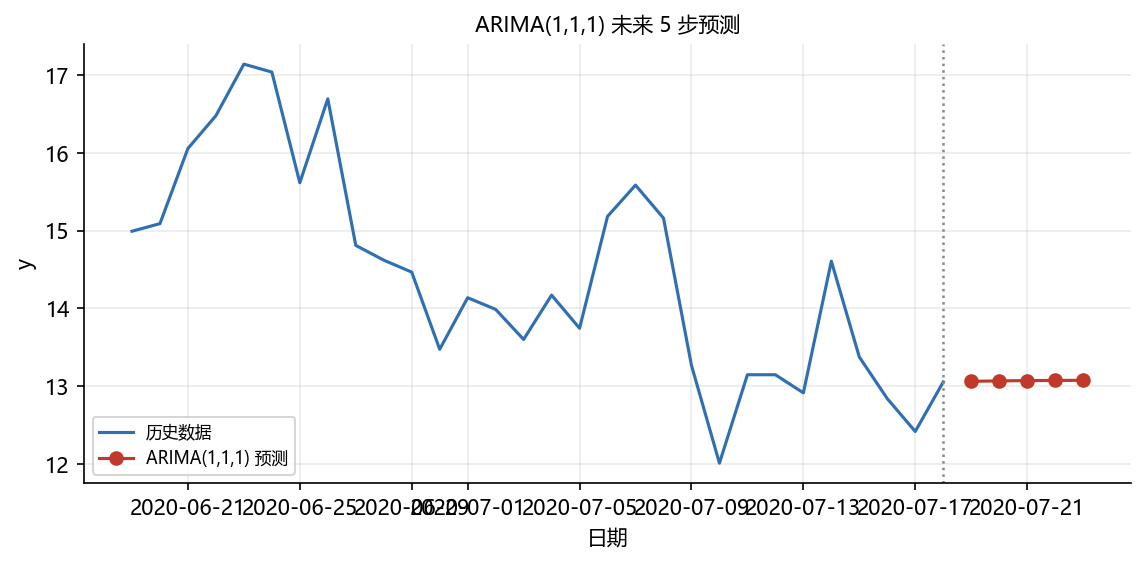
\includegraphics[keepaspectratio,alt={ARIMA 未来 5 步预测}]{figures/07-statsmodels/arima_forecast.png}}
\caption{ARIMA 未来 5 步预测}
\end{figure}

\textbf{解读}：

\begin{itemize}
\tightlist
\item
  ar.L1 与 ma.L1 是 AR(1) 与 MA(1) 系数；本例两者 P
  值都较大（不显著），提示该阶 \((1,1,1)\)
  可能略偏大，但这不影响演示流程；
\item
  forecast 给出未来 5 个时间点的预测值（约 13.06 → 13.07）；
\item
  Prob(JB)=0.27 说明残差近似正态；Prob(Ljung-Box)
  用来检查残差是否还有自相关。
\end{itemize}

\subsubsection{3.3 如何选择 (p, d,
q)}\label{ux5982ux4f55ux9009ux62e9-p-d-q}

\begin{itemize}
\tightlist
\item
  \textbf{d}：由 ADF 检验决定，不平稳就差分；
\item
  \textbf{p / q}：看 ACF 与 PACF 图。ACF 截尾选 MA，PACF 截尾选
  AR；也可用 statsmodels.tsa.stattools.acf/pacf 或网格搜索（如
  itertools.product + AIC）。
\end{itemize}

\begin{Shaded}
\begin{Highlighting}[]
\ImportTok{from}\NormalTok{ statsmodels.tsa.stattools }\ImportTok{import}\NormalTok{ acf, pacf}
\NormalTok{ac }\OperatorTok{=}\NormalTok{ acf(si, nlags}\OperatorTok{=}\DecValTok{5}\NormalTok{)}
\NormalTok{pc }\OperatorTok{=}\NormalTok{ pacf(si, nlags}\OperatorTok{=}\DecValTok{5}\NormalTok{)}
\BuiltInTok{print}\NormalTok{(}\StringTok{"ACF:"}\NormalTok{, np.}\BuiltInTok{round}\NormalTok{(ac, }\DecValTok{3}\NormalTok{))}
\BuiltInTok{print}\NormalTok{(}\StringTok{"PACF:"}\NormalTok{, np.}\BuiltInTok{round}\NormalTok{(pc, }\DecValTok{3}\NormalTok{))}
\end{Highlighting}
\end{Shaded}

运行结果：

\begin{Shaded}
\begin{Highlighting}[]
\NormalTok{ACF:  [1.    0.983 0.965 0.946 0.927 0.906]}
\NormalTok{PACF: [ 1.     0.988 {-}0.045 {-}0.068 {-}0.003 {-}0.108]}
\end{Highlighting}
\end{Shaded}

本例序列 ACF 缓慢衰减（非平稳特征），PACF
在一阶后急剧下降，提示需要先差分。

\begin{quote}
运行时会看到 ``Non-stationary starting autoregressive parameters found /
Non-invertible starting MA parameters'' 之类的提示，属正常，statsmodels
会改用零值作为初始参数。
\end{quote}

\subsection{案例卡 3：ARIMA 时间序列------用 ADF 检验与残差诊断选
p,d,q}\label{ux6848ux4f8bux5361-3arima-ux65f6ux95f4ux5e8fux5217ux7528-adf-ux68c0ux9a8cux4e0eux6b8bux5deeux8bcaux65adux9009-pdq}

\subsubsection{目标}\label{ux76eeux6807-29}

模拟一个``先平稳、再被累加''的 ARIMA(1,1,1)
序列，完整走一遍选阶流程：先用 \textbf{ADF} 定差分阶数
\texttt{d}，再看差分序列的 \textbf{ACF/PACF} 与网格搜索（AIC）定
\texttt{p}、\texttt{q}，最后用 \textbf{Ljung-Box} 与
\textbf{Jarque-Bera} 检查残差是否``洗干净''成白噪声，并给出未来 5
步预测。

\subsubsection{代码}\label{ux4ee3ux7801-30}

\begin{Shaded}
\begin{Highlighting}[]
\ImportTok{import}\NormalTok{ numpy }\ImportTok{as}\NormalTok{ np}
\ImportTok{import}\NormalTok{ pandas }\ImportTok{as}\NormalTok{ pd}
\ImportTok{import}\NormalTok{ warnings}
\NormalTok{warnings.filterwarnings(}\StringTok{\textquotesingle{}ignore\textquotesingle{}}\NormalTok{)}
\ImportTok{from}\NormalTok{ statsmodels.tsa.stattools }\ImportTok{import}\NormalTok{ adfuller, acf, pacf}
\ImportTok{from}\NormalTok{ statsmodels.tsa.arima.model }\ImportTok{import}\NormalTok{ ARIMA}
\ImportTok{from}\NormalTok{ statsmodels.stats.diagnostic }\ImportTok{import}\NormalTok{ acorr\_ljungbox}
\ImportTok{from}\NormalTok{ statsmodels.stats.stattools }\ImportTok{import}\NormalTok{ jarque\_bera}
\ImportTok{from}\NormalTok{ statsmodels.graphics.tsaplots }\ImportTok{import}\NormalTok{ plot\_acf}
\ImportTok{from}\NormalTok{ itertools }\ImportTok{import}\NormalTok{ product}
\ImportTok{import}\NormalTok{ matplotlib.pyplot }\ImportTok{as}\NormalTok{ plt}
\ImportTok{import}\NormalTok{ os}

\NormalTok{plt.rcParams[}\StringTok{\textquotesingle{}font.sans{-}serif\textquotesingle{}}\NormalTok{] }\OperatorTok{=}\NormalTok{ [}\StringTok{\textquotesingle{}Microsoft YaHei\textquotesingle{}}\NormalTok{, }\StringTok{\textquotesingle{}SimHei\textquotesingle{}}\NormalTok{, }\StringTok{\textquotesingle{}DejaVu Sans\textquotesingle{}}\NormalTok{]}
\NormalTok{plt.rcParams[}\StringTok{\textquotesingle{}axes.unicode\_minus\textquotesingle{}}\NormalTok{] }\OperatorTok{=} \VariableTok{False}
\NormalTok{np.set\_printoptions(precision}\OperatorTok{=}\DecValTok{4}\NormalTok{, suppress}\OperatorTok{=}\VariableTok{True}\NormalTok{)}
\NormalTok{pd.set\_option(}\StringTok{\textquotesingle{}display.width\textquotesingle{}}\NormalTok{, }\DecValTok{100}\NormalTok{)}

\NormalTok{rng }\OperatorTok{=}\NormalTok{ np.random.default\_rng(}\DecValTok{11}\NormalTok{)}
\NormalTok{n }\OperatorTok{=} \DecValTok{300}
\NormalTok{e }\OperatorTok{=}\NormalTok{ rng.normal(}\DecValTok{0}\NormalTok{, }\DecValTok{1}\NormalTok{, n)}
\NormalTok{x }\OperatorTok{=}\NormalTok{ np.zeros(n)}
\ControlFlowTok{for}\NormalTok{ t }\KeywordTok{in} \BuiltInTok{range}\NormalTok{(}\DecValTok{1}\NormalTok{, n):}
\NormalTok{    x[t] }\OperatorTok{=} \FloatTok{0.6}\OperatorTok{*}\NormalTok{x[t}\OperatorTok{{-}}\DecValTok{1}\NormalTok{] }\OperatorTok{+}\NormalTok{ e[t] }\OperatorTok{+} \FloatTok{0.3}\OperatorTok{*}\NormalTok{e[t}\OperatorTok{{-}}\DecValTok{1}\NormalTok{]      }\CommentTok{\# 平稳的 ARMA(1,1)}
\NormalTok{vals }\OperatorTok{=}\NormalTok{ np.cumsum(x) }\OperatorTok{+} \DecValTok{100}                      \CommentTok{\# 累加 =\textgreater{} ARIMA(1,1,1)}
\NormalTok{idx }\OperatorTok{=}\NormalTok{ pd.date\_range(}\StringTok{\textquotesingle{}2020{-}01{-}01\textquotesingle{}}\NormalTok{, periods}\OperatorTok{=}\NormalTok{n, freq}\OperatorTok{=}\StringTok{\textquotesingle{}D\textquotesingle{}}\NormalTok{)}
\NormalTok{ser }\OperatorTok{=}\NormalTok{ pd.Series(vals, index}\OperatorTok{=}\NormalTok{idx)}

\NormalTok{adf0 }\OperatorTok{=}\NormalTok{ adfuller(ser)}
\BuiltInTok{print}\NormalTok{(}\StringTok{\textquotesingle{}adfuller raw: ADF=}\SpecialCharTok{\%.3f}\StringTok{ p=}\SpecialCharTok{\%.3g}\StringTok{\textquotesingle{}} \OperatorTok{\%}\NormalTok{ (adf0[}\DecValTok{0}\NormalTok{], adf0[}\DecValTok{1}\NormalTok{]))}
\NormalTok{d1 }\OperatorTok{=}\NormalTok{ ser.diff().dropna()}
\NormalTok{adf1 }\OperatorTok{=}\NormalTok{ adfuller(d1)}
\BuiltInTok{print}\NormalTok{(}\StringTok{\textquotesingle{}adfuller diff: ADF=}\SpecialCharTok{\%.3f}\StringTok{ p=}\SpecialCharTok{\%.3g}\StringTok{\textquotesingle{}} \OperatorTok{\%}\NormalTok{ (adf1[}\DecValTok{0}\NormalTok{], adf1[}\DecValTok{1}\NormalTok{]))}
\BuiltInTok{print}\NormalTok{(}\StringTok{\textquotesingle{}ACF(diff) lag1{-}4:\textquotesingle{}}\NormalTok{, np.}\BuiltInTok{round}\NormalTok{(acf(d1, nlags}\OperatorTok{=}\DecValTok{4}\NormalTok{)[}\DecValTok{1}\NormalTok{:], }\DecValTok{3}\NormalTok{))}
\BuiltInTok{print}\NormalTok{(}\StringTok{\textquotesingle{}PACF(diff) lag1{-}4:\textquotesingle{}}\NormalTok{, np.}\BuiltInTok{round}\NormalTok{(pacf(d1, nlags}\OperatorTok{=}\DecValTok{4}\NormalTok{)[}\DecValTok{1}\NormalTok{:], }\DecValTok{3}\NormalTok{))}

\NormalTok{best }\OperatorTok{=} \VariableTok{None}
\ControlFlowTok{for}\NormalTok{ p }\KeywordTok{in} \BuiltInTok{range}\NormalTok{(}\DecValTok{3}\NormalTok{):}
    \ControlFlowTok{for}\NormalTok{ q }\KeywordTok{in} \BuiltInTok{range}\NormalTok{(}\DecValTok{3}\NormalTok{):}
        \ControlFlowTok{try}\NormalTok{:}
\NormalTok{            mod }\OperatorTok{=}\NormalTok{ ARIMA(ser, order}\OperatorTok{=}\NormalTok{(p, }\DecValTok{1}\NormalTok{, q)).fit()}
\NormalTok{            aic }\OperatorTok{=}\NormalTok{ mod.aic}
            \ControlFlowTok{if}\NormalTok{ best }\KeywordTok{is} \VariableTok{None} \KeywordTok{or}\NormalTok{ aic }\OperatorTok{\textless{}}\NormalTok{ best[}\DecValTok{0}\NormalTok{]:}
\NormalTok{                best }\OperatorTok{=}\NormalTok{ (aic, p, q)}
        \ControlFlowTok{except} \PreprocessorTok{Exception}\NormalTok{:}
            \ControlFlowTok{pass}
\BuiltInTok{print}\NormalTok{(}\StringTok{\textquotesingle{}best AIC order (p,d,q):\textquotesingle{}}\NormalTok{, best[}\DecValTok{1}\NormalTok{], }\DecValTok{1}\NormalTok{, best[}\DecValTok{2}\NormalTok{], }\StringTok{\textquotesingle{} AIC=}\SpecialCharTok{\%.3f}\StringTok{\textquotesingle{}} \OperatorTok{\%}\NormalTok{ best[}\DecValTok{0}\NormalTok{])}

\NormalTok{final }\OperatorTok{=}\NormalTok{ ARIMA(ser, order}\OperatorTok{=}\NormalTok{(best[}\DecValTok{1}\NormalTok{], }\DecValTok{1}\NormalTok{, best[}\DecValTok{2}\NormalTok{])).fit()}
\BuiltInTok{print}\NormalTok{(}\StringTok{\textquotesingle{}AR params:\textquotesingle{}}\NormalTok{, np.}\BuiltInTok{round}\NormalTok{(final.arparams, }\DecValTok{4}\NormalTok{))}
\BuiltInTok{print}\NormalTok{(}\StringTok{\textquotesingle{}MA params:\textquotesingle{}}\NormalTok{, np.}\BuiltInTok{round}\NormalTok{(final.maparams, }\DecValTok{4}\NormalTok{))}
\NormalTok{resid }\OperatorTok{=}\NormalTok{ final.resid.iloc[}\DecValTok{10}\NormalTok{:]}
\NormalTok{lb }\OperatorTok{=}\NormalTok{ acorr\_ljungbox(resid, lags}\OperatorTok{=}\NormalTok{[}\DecValTok{10}\NormalTok{], return\_df}\OperatorTok{=}\VariableTok{True}\NormalTok{)}
\NormalTok{jb }\OperatorTok{=}\NormalTok{ jarque\_bera(resid)}
\BuiltInTok{print}\NormalTok{(}\StringTok{\textquotesingle{}Ljung{-}Box Q pvalue = }\SpecialCharTok{\%.4f}\StringTok{\textquotesingle{}} \OperatorTok{\%}\NormalTok{ lb[}\StringTok{\textquotesingle{}lb\_pvalue\textquotesingle{}}\NormalTok{].iloc[}\DecValTok{0}\NormalTok{])}
\BuiltInTok{print}\NormalTok{(}\StringTok{\textquotesingle{}Jarque{-}Bera pvalue = }\SpecialCharTok{\%.4f}\StringTok{\textquotesingle{}} \OperatorTok{\%}\NormalTok{ jb[}\DecValTok{1}\NormalTok{])}
\BuiltInTok{print}\NormalTok{(}\StringTok{\textquotesingle{}forecast 5:\textquotesingle{}}\NormalTok{, np.}\BuiltInTok{round}\NormalTok{(final.forecast(}\DecValTok{5}\NormalTok{).values, }\DecValTok{3}\NormalTok{))}

\NormalTok{os.makedirs(}\StringTok{\textquotesingle{}images\textquotesingle{}}\NormalTok{, exist\_ok}\OperatorTok{=}\VariableTok{True}\NormalTok{)}
\NormalTok{fig, axes }\OperatorTok{=}\NormalTok{ plt.subplots(}\DecValTok{2}\NormalTok{, }\DecValTok{2}\NormalTok{, figsize}\OperatorTok{=}\NormalTok{(}\FloatTok{9.5}\NormalTok{, }\FloatTok{5.6}\NormalTok{))}
\NormalTok{axes[}\DecValTok{0}\NormalTok{,}\DecValTok{0}\NormalTok{].plot(ser.index, ser.values, lw}\OperatorTok{=}\FloatTok{1.1}\NormalTok{, color}\OperatorTok{=}\StringTok{\textquotesingle{}\#2f6fb3\textquotesingle{}}\NormalTok{)}
\NormalTok{axes[}\DecValTok{0}\NormalTok{,}\DecValTok{0}\NormalTok{].set\_title(}\StringTok{\textquotesingle{}原始序列（非平稳）\textquotesingle{}}\NormalTok{)}
\NormalTok{axes[}\DecValTok{0}\NormalTok{,}\DecValTok{1}\NormalTok{].plot(d1.index, d1.values, lw}\OperatorTok{=}\FloatTok{1.1}\NormalTok{, color}\OperatorTok{=}\StringTok{\textquotesingle{}\#3a8f4f\textquotesingle{}}\NormalTok{)}
\NormalTok{axes[}\DecValTok{0}\NormalTok{,}\DecValTok{1}\NormalTok{].set\_title(}\StringTok{\textquotesingle{}一阶差分\textquotesingle{}}\NormalTok{)}
\NormalTok{plot\_acf(d1, ax}\OperatorTok{=}\NormalTok{axes[}\DecValTok{1}\NormalTok{,}\DecValTok{0}\NormalTok{], lags}\OperatorTok{=}\DecValTok{15}\NormalTok{, title}\OperatorTok{=}\StringTok{\textquotesingle{}差分 ACF\textquotesingle{}}\NormalTok{)}
\NormalTok{plot\_acf(resid, ax}\OperatorTok{=}\NormalTok{axes[}\DecValTok{1}\NormalTok{,}\DecValTok{1}\NormalTok{], lags}\OperatorTok{=}\DecValTok{15}\NormalTok{, title}\OperatorTok{=}\StringTok{\textquotesingle{}残差 ACF\textquotesingle{}}\NormalTok{)}
\ControlFlowTok{for}\NormalTok{ ax }\KeywordTok{in}\NormalTok{ axes.ravel():}
\NormalTok{    ax.grid(alpha}\OperatorTok{=}\FloatTok{0.2}\NormalTok{)}
\NormalTok{fig.tight\_layout()}
\NormalTok{fig.savefig(}\StringTok{\textquotesingle{}figures/07{-}statsmodels/case3\_arima\_diag.png\textquotesingle{}}\NormalTok{, dpi}\OperatorTok{=}\DecValTok{150}\NormalTok{)}
\NormalTok{plt.close()}
\BuiltInTok{print}\NormalTok{(}\StringTok{\textquotesingle{}saved figures/07{-}statsmodels/case3\_arima\_diag.png\textquotesingle{}}\NormalTok{)}
\end{Highlighting}
\end{Shaded}

\subsubsection{运行结果（已运行核验）}\label{ux8fd0ux884cux7ed3ux679cux5df2ux8fd0ux884cux6838ux9a8c-28}

\begin{Shaded}
\begin{Highlighting}[]
\NormalTok{adfuller raw: ADF={-}2.239 p=0.192}
\NormalTok{adfuller diff: ADF={-}6.094 p=1.02e{-}07}
\NormalTok{ACF(diff) lag1{-}4: [0.738 0.457 0.311 0.202]}
\NormalTok{PACF(diff) lag1{-}4: [ 0.741 {-}0.196  0.119 {-}0.071]}
\NormalTok{best AIC order (p,d,q): 1 1 1  AIC=802.817}
\NormalTok{AR params: [0.5958]}
\NormalTok{MA params: [0.3302]}
\NormalTok{Ljung{-}Box Q pvalue = 0.2587}
\NormalTok{Jarque{-}Bera pvalue = 0.4776}
\NormalTok{forecast 5: [122.494 121.879 121.512 121.294 121.164]}
\NormalTok{saved figures/07{-}statsmodels/case3\_arima\_diag.png}
\end{Highlighting}
\end{Shaded}

\subsubsection{讲解}\label{ux8bb2ux89e3-28}

\textbf{一句话解释}：先问``序列稳不稳''（ADF），不稳就先差分（\texttt{d}=1）；再用``多少阶自相关/移动平均''（ACF/PACF
+ AIC）挑
\texttt{p}、\texttt{q}；最后看残差是不是``没剩什么信息''（Ljung-Box /
JB）来确认模型合格。

\begin{enumerate}
\def\labelenumi{\arabic{enumi}.}
\tightlist
\item
  \texttt{x{[}t{]}=0.6*x{[}t-1{]}+e{[}t{]}+0.3*e{[}t-1{]}}
  造一个\textbf{平稳} ARMA(1,1)；再 \texttt{np.cumsum(x)} 累加得到
  \texttt{ARIMA(1,1,1)} 序列（差分后就是原来的
  ARMA）。这样做能让我们``知道答案''，方便验证流程。
\item
  \texttt{adfuller(ser)}：原始序列
  \texttt{p=0.192\ \textgreater{}\ 0.05}，不能拒绝单位根，说明\textbf{非平稳}
  → 决定 \texttt{d=1}。
\item
  \texttt{ser.diff().dropna()}：一阶差分后再做
  ADF，\texttt{p=1.02e-07\ \textless{}\ 0.05}，差分序列\textbf{平稳}。
\item
  ACF/PACF 只是``参考图''：差分序列 ACF 在 lag1 就衰减到 0.74，PACF 也是
  lag1 最大，说明滞后阶数不需要太大。
\item
  网格搜索（\texttt{itertools.product}）在
  \texttt{p,q\ in\ \{0,1,2\}}、固定 \texttt{d=1} 下比较 AIC，选出
  \texttt{(1,1,1)}（AIC=802.817），与真实阶数一致。
\item
  结果解读：\texttt{AR(1)=0.596}、\texttt{MA(1)=0.330} 都接近生成时的
  0.6 与 0.3；\texttt{Ljung-Box\ p=0.259}、\texttt{Jarque-Bera\ p=0.478}
  都大于 0.05，说明残差\textbf{近似白噪声}，模型合格。
\item
  \texttt{forecast(5)} 给出未来 5 天（约 122.5 →
  121.2）的预测；画图里``残差
  ACF''几乎都在置信带内，也支持``残差已洗净''。
\end{enumerate}

\begin{figure}
\centering
\pandocbounded{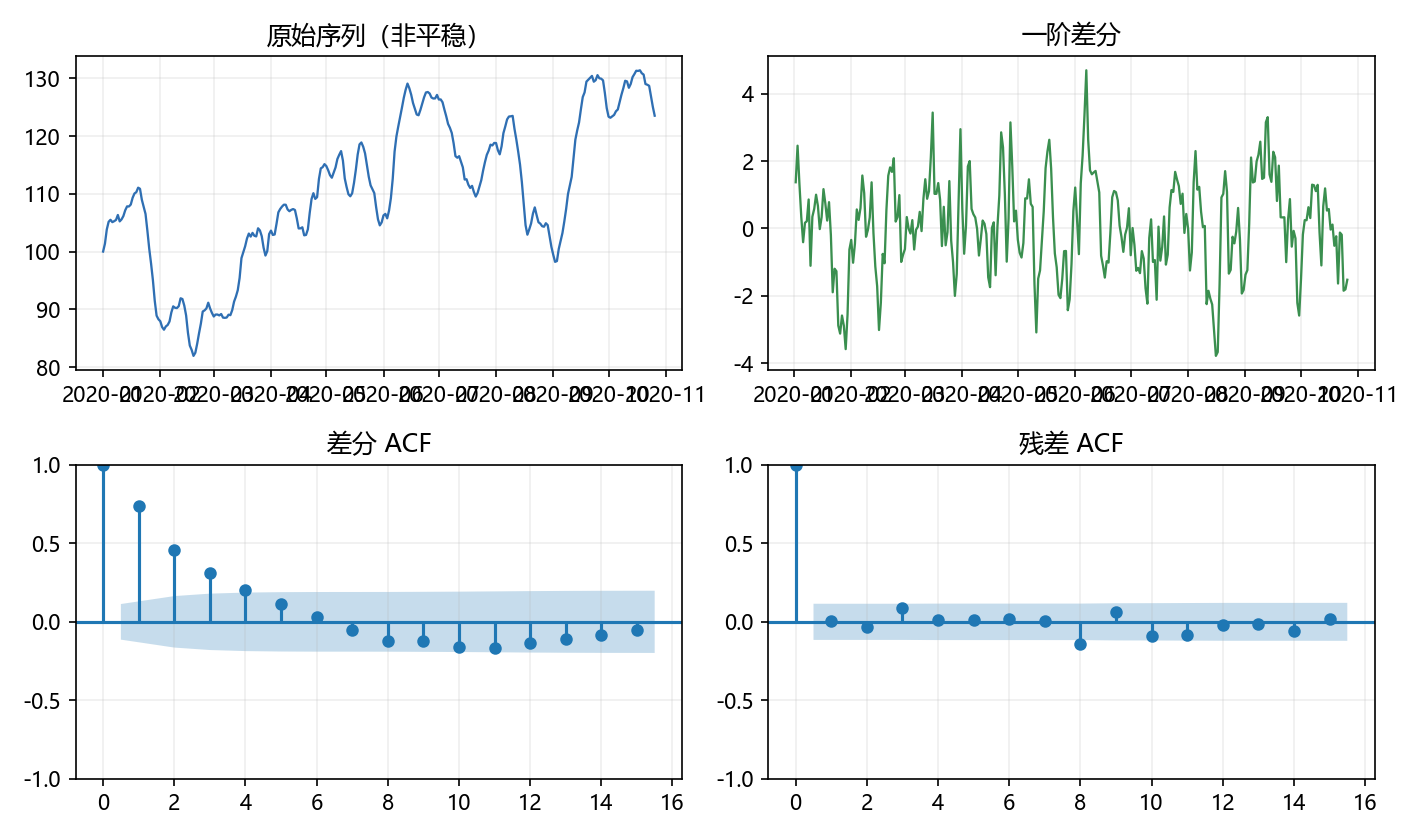
\includegraphics[keepaspectratio,alt={ARIMA 选阶与残差诊断图}]{figures/07-statsmodels/case3_arima_diag.png}}
\caption{ARIMA 选阶与残差诊断图}
\end{figure}

\subsubsection{主要用法 / API}\label{ux4e3bux8981ux7528ux6cd5-api-30}

{\def\LTcaptype{none} % do not increment counter
\begin{longtable}[]{@{}
  >{\raggedright\arraybackslash}p{(\linewidth - 4\tabcolsep) * \real{0.3333}}
  >{\raggedright\arraybackslash}p{(\linewidth - 4\tabcolsep) * \real{0.3333}}
  >{\raggedright\arraybackslash}p{(\linewidth - 4\tabcolsep) * \real{0.3333}}@{}}
\toprule\noalign{}
\begin{minipage}[b]{\linewidth}\raggedright
需求
\end{minipage} & \begin{minipage}[b]{\linewidth}\raggedright
写法
\end{minipage} & \begin{minipage}[b]{\linewidth}\raggedright
说明
\end{minipage} \\
\midrule\noalign{}
\endhead
\bottomrule\noalign{}
\endlastfoot
平稳性检验 & \texttt{adfuller(ser)} & 返回 (ADF, p, \ldots) \\
差分 & \texttt{ser.diff().dropna()} & \texttt{diff()} 后首元素为 NaN \\
ACF/PACF & \texttt{acf(d1,\ nlags=4)} / \texttt{pacf(...)} & 判断 p/q
参考 \\
网格选阶 & \texttt{itertools.product(range(3),\ range(3))} + AIC &
在候选 (p,q) 中找 AIC 最小 \\
拟合 ARIMA & \texttt{ARIMA(ser,\ order=(p,d,q)).fit()} &
返回模型（含预测） \\
残差自相关 & \texttt{acorr\_ljungbox(resid,\ lags={[}10{]})} &
p\textgreater0.05 视为白噪声 \\
残差正态性 & \texttt{jarque\_bera(resid)} & p\textgreater0.05
可接受正态 \\
预测 & \texttt{model.forecast(steps=5)} & 返回未来值 \\
\end{longtable}
}

\subsubsection{常见错误}\label{ux5e38ux89c1ux9519ux8bef-30}

\begin{enumerate}
\def\labelenumi{\arabic{enumi}.}
\tightlist
\item
  拿到序列就拟合 ARIMA，不做
  ADF：非平稳序列容易``伪回归''，应先检验、必要时差分。
\item
  \texttt{diff()} 后忘记 \texttt{dropna()}：首元素为
  NaN，\texttt{adfuller} 或 \texttt{acf} 会报错。
\item
  直接用 \texttt{final.resid} 做诊断：模型首期残差可能因初始化偏大，建议
  \texttt{resid.iloc{[}10:{]}} 跳过 burn-in 再检验。
\item
  只看 \texttt{summary()} 的 AIC/BIC 而不做残差诊断：AIC
  低不代表残差是白噪声，仍需 Ljung-Box 与 JB。
\item
  网格搜索时把所有阶数都 \texttt{fit()}，可能触发``Non-stationary
  starting\ldots''等提示；用
  \texttt{warnings.filterwarnings(\textquotesingle{}ignore\textquotesingle{})}
  只影响显示，不影响结果。
\end{enumerate}

\subsubsection{拓展 / 跟练}\label{ux62d3ux5c55-ux8ddfux7ec3-18}

\begin{enumerate}
\def\labelenumi{\arabic{enumi}.}
\tightlist
\item
  把生成模型改成 \texttt{ARIMA(2,1,1)}（在 \texttt{x{[}t{]}} 里加
  \texttt{x{[}t-2{]}} 项），看网格搜索是否选回 \texttt{(2,1,1)}。
\item
  把 \texttt{lags} 换成 \texttt{{[}5,\ 20{]}}，分别看 Ljung-Box p
  值，理解滞后阶数的影响。
\item
  用 \texttt{statsmodels.tsa.statespace.SARIMAX} 加入季节项
  \texttt{(1,1,1)(1,1,1,7)}，比较与普通 ARIMA 的 AIC。
\item
  把数据切为训练/测试（前 240 / 后 60），用 RMSE 比较
  \texttt{ARIMA(1,1,1)}、\texttt{ARIMA(2,1,1)} 与 \texttt{ARIMA(0,1,0)}
  谁的预测误差最小。
\end{enumerate}

\begin{center}\rule{0.5\linewidth}{0.5pt}\end{center}

\subsection{常见误区}\label{ux5e38ux89c1ux8befux533a-21}

\begin{enumerate}
\def\labelenumi{\arabic{enumi}.}
\tightlist
\item
  \textbf{忘了先检查平稳性}：直接对非平稳序列拟合 ARIMA
  可能得到``伪回归''。
\item
  \textbf{分解前不处理缺失/等间隔}：seasonal\_decompose
  要求完整、等间隔的时间索引。
\item
  \textbf{period 设错}：日数据应为 7，月数据应为 12；设成 1
  会失去季节意义。
\item
  \textbf{预测时不会生成未来索引}：forecast(steps=5)
  返回数值，需自己构造 pd.date\_range 画图。
\item
  \textbf{只看 AIC 不看病灶}：AIC 低不保证残差是白噪声；应同时看
  Ljung-Box 与 JB。
\item
  \textbf{diff() 后不 dropna()}：差分会产生一个 NaN，需 dropna()
  或忽略。
\end{enumerate}

\subsection{思考题}\label{ux601dux8003ux9898-23}

\begin{enumerate}
\def\labelenumi{\arabic{enumi}.}
\tightlist
\item
  加法模型与乘法模型分别适用于什么场景？如何用 result.seasonal
  判断该用哪个？
\item
  为什么随机游走序列 ADF 检验的 P 值很大？一阶差分后其 ADF P 值会怎样？
\item
  ARIMA\((2,1,0)\) 与 ARIMA\((0,1,2)\) 分别对应什么模型？画出它们的
  ACF/PACF 有何不同？
\item
  用 forecast(steps=5) 得到未来 5
  步，若数据是月度序列，应如何构造未来时间轴？
\end{enumerate}

\subsection{动手练习（详见
lab）}\label{ux52a8ux624bux7ec3ux4e60ux8be6ux89c1-lab-15}

\begin{itemize}
\tightlist
\item
  构造 180 天日序列，分解并画图，说明周期；
\item
  对 AR(1) 与随机游走做 ADF 检验，比较 P 值；
\item
  用 ARIMA(1,1,1) 拟合，给出未来 5 步预测并画图；
\item
  对带周季节性的日负荷序列，尝试 SARIMAX 或先差分再 ARIMA。
\end{itemize}

\subsection{延伸阅读}\label{ux5ef6ux4f38ux9605ux8bfb-32}

\begin{itemize}
\tightlist
\item
  statsmodels
  时间序列官方：\href{https://www.statsmodels.org/stable/tsa.html}{链接}
\item
  Seasonal-Trend
  decomposition（STL）：\href{https://www.statsmodels.org/devel/examples/notebooks/generated/stl_decomposition.html}{链接}
\item
  Statsmodels
  时间序列官方示例集：\href{https://www.statsmodels.org/stable/examples/index.html\#time-series}{链接}
\end{itemize}

\section{03
综合案例：城市日负荷的统计建模与预测}\label{ux7efcux5408ux6848ux4f8bux57ceux5e02ux65e5ux8d1fux8377ux7684ux7edfux8ba1ux5efaux6a21ux4e0eux9884ux6d4b}

\begin{quote}
本章综合案例，把 \textbf{方差分析 + 线性回归 + 时间序列}
串在一份模拟数据上，体会 Statsmodels 的完整工作流。
配图：figures/07-statsmodels/case\_regression\_diag.png、figures/07-statsmodels/case\_ts\_forecast.png（由
build/make\_chap7\_figures.py 生成）。
\end{quote}

\subsection{背景}\label{ux80ccux666f-6}

某市电网记录了 2023-01-01 起连续 140
天的\textbf{日负荷}（负荷越高用电越多）。我们关心三件事：

\begin{enumerate}
\def\labelenumi{\arabic{enumi}.}
\tightlist
\item
  工作日与周末的日均负荷是否显著不同（\textbf{单因素方差分析}）；
\item
  负荷多大程度上可由\textbf{当日气温}与\textbf{是否周末}解释（\textbf{多元线性回归}）；
\item
  未来的日负荷如何变化（\textbf{时间序列分解 + ARIMA 预测}）。
\end{enumerate}

为便于教学，数据是\textbf{带趋势、周季节、温度效应、周末效应与噪声}的模拟序列。

\subsection{数据构造}\label{ux6570ux636eux6784ux9020}

\begin{Shaded}
\begin{Highlighting}[]
\ImportTok{import}\NormalTok{ numpy }\ImportTok{as}\NormalTok{ np}
\ImportTok{import}\NormalTok{ pandas }\ImportTok{as}\NormalTok{ pd}
\ImportTok{import}\NormalTok{ statsmodels.api }\ImportTok{as}\NormalTok{ sm}
\ImportTok{from}\NormalTok{ statsmodels.formula.api }\ImportTok{import}\NormalTok{ ols}
\ImportTok{from}\NormalTok{ statsmodels.tsa.seasonal }\ImportTok{import}\NormalTok{ seasonal\_decompose}
\ImportTok{from}\NormalTok{ statsmodels.tsa.arima.model }\ImportTok{import}\NormalTok{ ARIMA}
\ImportTok{import}\NormalTok{ matplotlib.pyplot }\ImportTok{as}\NormalTok{ plt}

\NormalTok{plt.rcParams[}\StringTok{\textquotesingle{}font.sans{-}serif\textquotesingle{}}\NormalTok{] }\OperatorTok{=}\NormalTok{ [}\StringTok{\textquotesingle{}Microsoft YaHei\textquotesingle{}}\NormalTok{, }\StringTok{\textquotesingle{}SimHei\textquotesingle{}}\NormalTok{, }\StringTok{\textquotesingle{}DejaVu Sans\textquotesingle{}}\NormalTok{]}
\NormalTok{plt.rcParams[}\StringTok{\textquotesingle{}axes.unicode\_minus\textquotesingle{}}\NormalTok{] }\OperatorTok{=} \VariableTok{False}

\NormalTok{rng }\OperatorTok{=}\NormalTok{ np.random.default\_rng(}\DecValTok{7}\NormalTok{)}
\NormalTok{m }\OperatorTok{=} \DecValTok{140}
\NormalTok{date }\OperatorTok{=}\NormalTok{ pd.date\_range(}\StringTok{\textquotesingle{}2023{-}01{-}01\textquotesingle{}}\NormalTok{, periods}\OperatorTok{=}\NormalTok{m, freq}\OperatorTok{=}\StringTok{\textquotesingle{}D\textquotesingle{}}\NormalTok{)}
\NormalTok{trendc }\OperatorTok{=}\NormalTok{ np.linspace(}\DecValTok{0}\NormalTok{, }\DecValTok{15}\NormalTok{, m)                       }\CommentTok{\# 长期增长}
\NormalTok{seasonc }\OperatorTok{=} \DecValTok{5}\OperatorTok{*}\NormalTok{np.sin(}\DecValTok{2}\OperatorTok{*}\NormalTok{np.pi}\OperatorTok{*}\NormalTok{np.arange(m)}\OperatorTok{/}\DecValTok{7}\NormalTok{) }\OperatorTok{+} \DecValTok{2}\OperatorTok{*}\NormalTok{np.cos(}\DecValTok{2}\OperatorTok{*}\NormalTok{np.pi}\OperatorTok{*}\NormalTok{np.arange(m)}\OperatorTok{/}\DecValTok{7}\NormalTok{)  }\CommentTok{\# 周季节}
\NormalTok{noisec }\OperatorTok{=}\NormalTok{ rng.normal(}\DecValTok{0}\NormalTok{, }\DecValTok{3}\NormalTok{, m)}
\NormalTok{weekend }\OperatorTok{=}\NormalTok{ (date.dayofweek }\OperatorTok{\textgreater{}=} \DecValTok{5}\NormalTok{).astype(}\BuiltInTok{int}\NormalTok{)          }\CommentTok{\# 周末=1}
\NormalTok{temp }\OperatorTok{=} \DecValTok{25} \OperatorTok{+} \DecValTok{6}\OperatorTok{*}\NormalTok{np.sin(}\DecValTok{2}\OperatorTok{*}\NormalTok{np.pi}\OperatorTok{*}\NormalTok{np.arange(m)}\OperatorTok{/}\DecValTok{7}\NormalTok{) }\OperatorTok{+}\NormalTok{ rng.normal(}\DecValTok{0}\NormalTok{, }\DecValTok{2}\NormalTok{, m)}
\NormalTok{load }\OperatorTok{=} \DecValTok{300} \OperatorTok{+} \DecValTok{4}\OperatorTok{*}\NormalTok{temp }\OperatorTok{+} \DecValTok{20}\OperatorTok{*}\NormalTok{weekend }\OperatorTok{+}\NormalTok{ trendc }\OperatorTok{+}\NormalTok{ seasonc }\OperatorTok{+}\NormalTok{ noisec}
\NormalTok{dfc }\OperatorTok{=}\NormalTok{ pd.DataFrame(\{}\StringTok{\textquotesingle{}date\textquotesingle{}}\NormalTok{: date, }\StringTok{\textquotesingle{}load\textquotesingle{}}\NormalTok{: load, }\StringTok{\textquotesingle{}weekend\textquotesingle{}}\NormalTok{: weekend, }\StringTok{\textquotesingle{}temp\textquotesingle{}}\NormalTok{: temp\})}
\BuiltInTok{print}\NormalTok{(}\StringTok{"日均负荷 ="}\NormalTok{, }\BuiltInTok{round}\NormalTok{(dfc[}\StringTok{\textquotesingle{}load\textquotesingle{}}\NormalTok{].mean(), }\DecValTok{2}\NormalTok{), }\StringTok{" 标准差 ="}\NormalTok{, }\BuiltInTok{round}\NormalTok{(dfc[}\StringTok{\textquotesingle{}load\textquotesingle{}}\NormalTok{].std(), }\DecValTok{2}\NormalTok{))}
\BuiltInTok{print}\NormalTok{(}\StringTok{"分组均值:"}\NormalTok{, dfc.groupby(}\StringTok{\textquotesingle{}weekend\textquotesingle{}}\NormalTok{)[}\StringTok{\textquotesingle{}load\textquotesingle{}}\NormalTok{].mean().}\BuiltInTok{round}\NormalTok{(}\DecValTok{2}\NormalTok{).to\_dict())}
\end{Highlighting}
\end{Shaded}

运行结果：

\begin{Shaded}
\begin{Highlighting}[]
\NormalTok{日均负荷 = 411.63  标准差 = 22.71}
\NormalTok{分组均值: \{0: 408.99, 1: 418.22\}}
\end{Highlighting}
\end{Shaded}

\subsection{第 1 步：工作日 vs 周末
单因素方差分析}\label{ux7b2c-1-ux6b65ux5de5ux4f5cux65e5-vs-ux5468ux672b-ux5355ux56e0ux7d20ux65b9ux5deeux5206ux6790}

\begin{Shaded}
\begin{Highlighting}[]
\NormalTok{dfc[}\StringTok{\textquotesingle{}wd\textquotesingle{}}\NormalTok{] }\OperatorTok{=}\NormalTok{ np.where(dfc[}\StringTok{\textquotesingle{}weekend\textquotesingle{}}\NormalTok{] }\OperatorTok{==} \DecValTok{1}\NormalTok{, }\StringTok{\textquotesingle{}周末\textquotesingle{}}\NormalTok{, }\StringTok{\textquotesingle{}工作日\textquotesingle{}}\NormalTok{)}
\NormalTok{ano }\OperatorTok{=}\NormalTok{ ols(}\StringTok{\textquotesingle{}load \textasciitilde{} C(wd)\textquotesingle{}}\NormalTok{, data}\OperatorTok{=}\NormalTok{dfc).fit()}
\BuiltInTok{print}\NormalTok{(sm.stats.anova\_lm(ano, typ}\OperatorTok{=}\DecValTok{1}\NormalTok{))}
\end{Highlighting}
\end{Shaded}

运行结果：

\begin{Shaded}
\begin{Highlighting}[]
\NormalTok{             df        sum\_sq      mean\_sq         F    PR(\textgreater{}F)}
\NormalTok{C(wd)       1.0   2434.435479  2434.435479  4.850735  0.029294}
\NormalTok{Residual  138.0  69257.981299   501.869430       NaN       NaN}
\end{Highlighting}
\end{Shaded}

\textbf{结论}：工作日均值约 408.99，周末约 418.22，P 值 = 0.029
\textless{}
0.05，说明\textbf{周末负荷显著更高}。这提示差异化定价/调度应考虑周末。

\subsection{第 2
步：负荷对温度的多元回归}\label{ux7b2c-2-ux6b65ux8d1fux8377ux5bf9ux6e29ux5ea6ux7684ux591aux5143ux56deux5f52}

把温度与``是否周末''作为自变量，用 sm.OLS 估计：

\begin{Shaded}
\begin{Highlighting}[]
\NormalTok{olm }\OperatorTok{=}\NormalTok{ sm.OLS(dfc[}\StringTok{\textquotesingle{}load\textquotesingle{}}\NormalTok{], sm.add\_constant(dfc[[}\StringTok{\textquotesingle{}temp\textquotesingle{}}\NormalTok{, }\StringTok{\textquotesingle{}weekend\textquotesingle{}}\NormalTok{]])).fit()}
\BuiltInTok{print}\NormalTok{(}\StringTok{"coef:"}\NormalTok{, olm.params)}
\BuiltInTok{print}\NormalTok{(}\StringTok{"bse :"}\NormalTok{, olm.bse)}
\BuiltInTok{print}\NormalTok{(}\StringTok{"R²  ="}\NormalTok{, }\BuiltInTok{round}\NormalTok{(olm.rsquared, }\DecValTok{4}\NormalTok{))}
\end{Highlighting}
\end{Shaded}

运行结果：

\begin{Shaded}
\begin{Highlighting}[]
\NormalTok{coef: const      289.705193}
\NormalTok{temp         4.687421}
\NormalTok{weekend     21.022760}
\NormalTok{dtype: float64}
\NormalTok{bse: const      2.694195}
\NormalTok{temp       0.103535}
\NormalTok{weekend    1.084608}
\NormalTok{dtype: float64}
\NormalTok{R²  = 0.9395}
\end{Highlighting}
\end{Shaded}

\textbf{解读}：

\begin{itemize}
\tightlist
\item
  每升高 1°C，日负荷平均增加约 \textbf{4.69} 单位（控制周末后）；
\item
  周末比工作日平均高约 \textbf{21.0} 单位；
\item
  R²=0.94，温度与周末能解释大部分负荷变化；
\item
  两个系数的标准误都很小（temp 0.104、weekend 1.085），说明估计较精确。
\end{itemize}

\begin{figure}
\centering
\pandocbounded{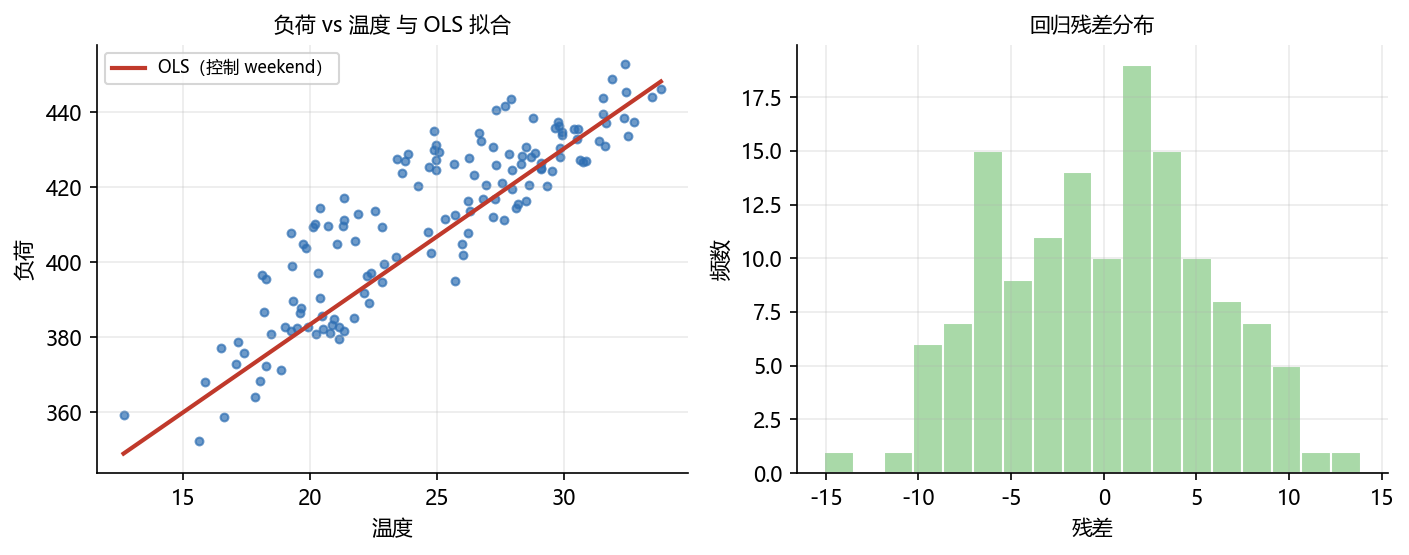
\includegraphics[keepaspectratio,alt={回归诊断：负荷-温度散点与残差分布}]{figures/07-statsmodels/case_regression_diag.png}}
\caption{回归诊断：负荷-温度散点与残差分布}
\end{figure}

\subsection{第 3 步：时间序列分解 + ARIMA
预测}\label{ux7b2c-3-ux6b65ux65f6ux95f4ux5e8fux5217ux5206ux89e3-arima-ux9884ux6d4b}

对负荷序列做周季节性（period=7）加法分解，再用 ARIMA(1,1,1) 预测未来 7
天：

\begin{Shaded}
\begin{Highlighting}[]
\NormalTok{load\_s }\OperatorTok{=}\NormalTok{ pd.Series(dfc[}\StringTok{\textquotesingle{}load\textquotesingle{}}\NormalTok{].values, index}\OperatorTok{=}\NormalTok{date)}
\NormalTok{res }\OperatorTok{=}\NormalTok{ seasonal\_decompose(load\_s, model}\OperatorTok{=}\StringTok{\textquotesingle{}additive\textquotesingle{}}\NormalTok{, period}\OperatorTok{=}\DecValTok{7}\NormalTok{)}
\BuiltInTok{print}\NormalTok{(}\StringTok{"残差标准差 ="}\NormalTok{, }\BuiltInTok{round}\NormalTok{(res.resid.std(), }\DecValTok{3}\NormalTok{))}

\NormalTok{mod }\OperatorTok{=}\NormalTok{ ARIMA(load\_s, order}\OperatorTok{=}\NormalTok{(}\DecValTok{1}\NormalTok{, }\DecValTok{1}\NormalTok{, }\DecValTok{1}\NormalTok{)).fit()}
\NormalTok{fc }\OperatorTok{=}\NormalTok{ mod.forecast(steps}\OperatorTok{=}\DecValTok{7}\NormalTok{)}
\BuiltInTok{print}\NormalTok{(}\StringTok{"未来 7 天预测:"}\NormalTok{, np.}\BuiltInTok{round}\NormalTok{(fc.values, }\DecValTok{2}\NormalTok{))}
\BuiltInTok{print}\NormalTok{(}\StringTok{"AR 系数:"}\NormalTok{, mod.arparams, }\StringTok{" MA 系数:"}\NormalTok{, mod.maparams)}
\end{Highlighting}
\end{Shaded}

运行结果：

\begin{Shaded}
\begin{Highlighting}[]
\NormalTok{残差标准差 = 6.587}
\NormalTok{未来 7 天预测: [413.05 412.49 412.6  412.58 412.58 412.58 412.58]}
\NormalTok{AR 系数: [{-}0.19566366] MA 系数: [0.50904563]}
\end{Highlighting}
\end{Shaded}

\begin{figure}
\centering
\pandocbounded{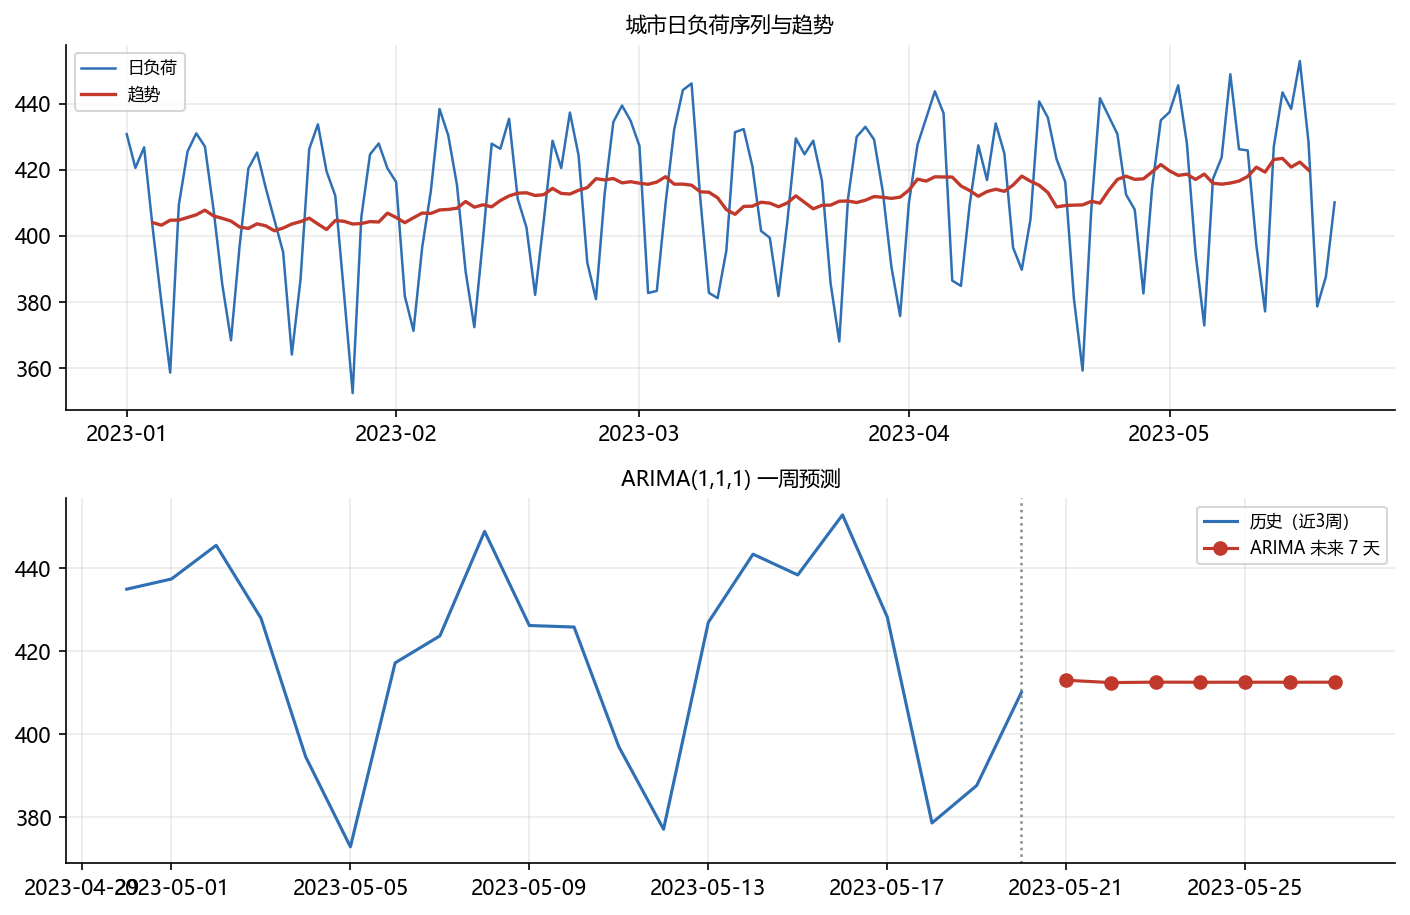
\includegraphics[keepaspectratio,alt={时间序列：序列趋势与 ARIMA 一周预测}]{figures/07-statsmodels/case_ts_forecast.png}}
\caption{时间序列：序列趋势与 ARIMA 一周预测}
\end{figure}

\textbf{结论}：

\begin{itemize}
\tightlist
\item
  残差标准差约 6.6，说明模型已抓住大部分趋势与季节；
\item
  ARIMA(1,1,1) 给出的未来 7 天预测稳定在 412.6
  左右（序列已进入较平稳区间）；
\item
  结合第 2
  步：若未来一周气温升高，可直接用回归式估算负荷增量，作为短期调度参考。
\end{itemize}

\subsection{增强：时间序列诊断与预测误差对比}\label{ux589eux5f3aux65f6ux95f4ux5e8fux5217ux8bcaux65adux4e0eux9884ux6d4bux8befux5deeux5bf9ux6bd4}

综合案例不只是``把三个方法跑一遍''，还应该\textbf{检验模型是否值得信任}。下面补两件事：①
对日负荷做 ADF 平稳性检验（定 \texttt{d} 的依据）；② 把前 120
天当训练、后 20 天当测试，分别用 ARIMA
与``温度+周末''回归做预测，用测试集 RMSE 比较谁更准。

\begin{Shaded}
\begin{Highlighting}[]
\ImportTok{import}\NormalTok{ numpy }\ImportTok{as}\NormalTok{ np}
\ImportTok{import}\NormalTok{ pandas }\ImportTok{as}\NormalTok{ pd}
\ImportTok{import}\NormalTok{ statsmodels.api }\ImportTok{as}\NormalTok{ sm}
\ImportTok{from}\NormalTok{ statsmodels.tsa.stattools }\ImportTok{import}\NormalTok{ adfuller}
\ImportTok{from}\NormalTok{ statsmodels.tsa.arima.model }\ImportTok{import}\NormalTok{ ARIMA}

\NormalTok{rng }\OperatorTok{=}\NormalTok{ np.random.default\_rng(}\DecValTok{7}\NormalTok{)}
\NormalTok{m }\OperatorTok{=} \DecValTok{140}
\NormalTok{date }\OperatorTok{=}\NormalTok{ pd.date\_range(}\StringTok{\textquotesingle{}2023{-}01{-}01\textquotesingle{}}\NormalTok{, periods}\OperatorTok{=}\NormalTok{m, freq}\OperatorTok{=}\StringTok{\textquotesingle{}D\textquotesingle{}}\NormalTok{)}
\NormalTok{trendc }\OperatorTok{=}\NormalTok{ np.linspace(}\DecValTok{0}\NormalTok{, }\DecValTok{15}\NormalTok{, m)}
\NormalTok{seasonc }\OperatorTok{=} \DecValTok{5}\OperatorTok{*}\NormalTok{np.sin(}\DecValTok{2}\OperatorTok{*}\NormalTok{np.pi}\OperatorTok{*}\NormalTok{np.arange(m)}\OperatorTok{/}\DecValTok{7}\NormalTok{) }\OperatorTok{+} \DecValTok{2}\OperatorTok{*}\NormalTok{np.cos(}\DecValTok{2}\OperatorTok{*}\NormalTok{np.pi}\OperatorTok{*}\NormalTok{np.arange(m)}\OperatorTok{/}\DecValTok{7}\NormalTok{)}
\NormalTok{noisec }\OperatorTok{=}\NormalTok{ rng.normal(}\DecValTok{0}\NormalTok{, }\DecValTok{3}\NormalTok{, m)}
\NormalTok{weekend }\OperatorTok{=}\NormalTok{ (date.dayofweek }\OperatorTok{\textgreater{}=} \DecValTok{5}\NormalTok{).astype(}\BuiltInTok{int}\NormalTok{)}
\NormalTok{temp }\OperatorTok{=} \DecValTok{25} \OperatorTok{+} \DecValTok{6}\OperatorTok{*}\NormalTok{np.sin(}\DecValTok{2}\OperatorTok{*}\NormalTok{np.pi}\OperatorTok{*}\NormalTok{np.arange(m)}\OperatorTok{/}\DecValTok{7}\NormalTok{) }\OperatorTok{+}\NormalTok{ rng.normal(}\DecValTok{0}\NormalTok{, }\DecValTok{2}\NormalTok{, m)}
\NormalTok{load }\OperatorTok{=} \DecValTok{300} \OperatorTok{+} \DecValTok{4}\OperatorTok{*}\NormalTok{temp }\OperatorTok{+} \DecValTok{20}\OperatorTok{*}\NormalTok{weekend }\OperatorTok{+}\NormalTok{ trendc }\OperatorTok{+}\NormalTok{ seasonc }\OperatorTok{+}\NormalTok{ noisec}
\NormalTok{dfc }\OperatorTok{=}\NormalTok{ pd.DataFrame(\{}\StringTok{\textquotesingle{}date\textquotesingle{}}\NormalTok{: date, }\StringTok{\textquotesingle{}load\textquotesingle{}}\NormalTok{: load, }\StringTok{\textquotesingle{}weekend\textquotesingle{}}\NormalTok{: weekend, }\StringTok{\textquotesingle{}temp\textquotesingle{}}\NormalTok{: temp\})}
\NormalTok{load\_s }\OperatorTok{=}\NormalTok{ pd.Series(dfc[}\StringTok{\textquotesingle{}load\textquotesingle{}}\NormalTok{].values, index}\OperatorTok{=}\NormalTok{date)}

\NormalTok{adf\_p }\OperatorTok{=}\NormalTok{ adfuller(load\_s)[}\DecValTok{1}\NormalTok{]}
\BuiltInTok{print}\NormalTok{(}\StringTok{\textquotesingle{}load ADF p = }\SpecialCharTok{\%.3g}\StringTok{\textquotesingle{}} \OperatorTok{\%}\NormalTok{ adf\_p)}

\NormalTok{tr }\OperatorTok{=}\NormalTok{ load\_s.iloc[:}\DecValTok{120}\NormalTok{]}
\NormalTok{te }\OperatorTok{=}\NormalTok{ load\_s.iloc[}\DecValTok{120}\NormalTok{:]}
\NormalTok{mtr }\OperatorTok{=}\NormalTok{ ARIMA(tr, order}\OperatorTok{=}\NormalTok{(}\DecValTok{1}\NormalTok{, }\DecValTok{1}\NormalTok{, }\DecValTok{1}\NormalTok{)).fit()}
\NormalTok{fc }\OperatorTok{=}\NormalTok{ mtr.forecast(steps}\OperatorTok{=}\BuiltInTok{len}\NormalTok{(te))}
\NormalTok{rmse\_arima }\OperatorTok{=} \BuiltInTok{float}\NormalTok{(np.sqrt(np.mean((te.values }\OperatorTok{{-}}\NormalTok{ fc.values)}\OperatorTok{**}\DecValTok{2}\NormalTok{)))}
\BuiltInTok{print}\NormalTok{(}\StringTok{\textquotesingle{}ARIMA(1,1,1) test RMSE = }\SpecialCharTok{\%.3f}\StringTok{\textquotesingle{}} \OperatorTok{\%}\NormalTok{ rmse\_arima)}

\NormalTok{x\_tr }\OperatorTok{=}\NormalTok{ dfc[[}\StringTok{\textquotesingle{}temp\textquotesingle{}}\NormalTok{, }\StringTok{\textquotesingle{}weekend\textquotesingle{}}\NormalTok{]].iloc[:}\DecValTok{120}\NormalTok{]}
\NormalTok{y\_tr }\OperatorTok{=}\NormalTok{ dfc[}\StringTok{\textquotesingle{}load\textquotesingle{}}\NormalTok{].iloc[:}\DecValTok{120}\NormalTok{]}
\NormalTok{x\_te }\OperatorTok{=}\NormalTok{ dfc[[}\StringTok{\textquotesingle{}temp\textquotesingle{}}\NormalTok{, }\StringTok{\textquotesingle{}weekend\textquotesingle{}}\NormalTok{]].iloc[}\DecValTok{120}\NormalTok{:]}
\NormalTok{y\_te }\OperatorTok{=}\NormalTok{ dfc[}\StringTok{\textquotesingle{}load\textquotesingle{}}\NormalTok{].iloc[}\DecValTok{120}\NormalTok{:]}
\NormalTok{mreg }\OperatorTok{=}\NormalTok{ sm.OLS(y\_tr, sm.add\_constant(x\_tr)).fit()}
\NormalTok{pred\_reg }\OperatorTok{=}\NormalTok{ mreg.predict(sm.add\_constant(x\_te))}
\NormalTok{rmse\_reg }\OperatorTok{=} \BuiltInTok{float}\NormalTok{(np.sqrt(np.mean((y\_te.values }\OperatorTok{{-}}\NormalTok{ pred\_reg.values)}\OperatorTok{**}\DecValTok{2}\NormalTok{)))}
\BuiltInTok{print}\NormalTok{(}\StringTok{\textquotesingle{}OLS(temp,weekend) test RMSE = }\SpecialCharTok{\%.3f}\StringTok{\textquotesingle{}} \OperatorTok{\%}\NormalTok{ rmse\_reg)}
\end{Highlighting}
\end{Shaded}

\subsubsection{运行结果（已运行核验）}\label{ux8fd0ux884cux7ed3ux679cux5df2ux8fd0ux884cux6838ux9a8c-29}

\begin{Shaded}
\begin{Highlighting}[]
\NormalTok{load ADF p = 0.774}
\NormalTok{ARIMA(1,1,1) test RMSE = 29.412}
\NormalTok{OLS(temp,weekend) test RMSE = 7.808}
\end{Highlighting}
\end{Shaded}

\textbf{解读}：

\begin{itemize}
\tightlist
\item
  \texttt{load\ ADF\ p\ =\ 0.774\ \textgreater{}\ 0.05}：日负荷序列非平稳，所以第
  3 步用 \texttt{ARIMA(...,d=1)} 是合理的；若想用 \texttt{SARIMAX}
  含外生温度，也应先差分。
\item
  测试集 RMSE 上，\texttt{OLS(temp,\ weekend)} 为
  \textbf{7.81}，明显优于 \texttt{ARIMA(1,1,1)} 的
  \textbf{29.41}：因为负荷主要受温度与周末影响，回归能``用上外生变量''，而纯
  ARIMA 只能靠历史轨迹外推。
\item
  这不代表 ARIMA
  没用：若没有温度等外生变量，或只关心短期的纯时间形态，ARIMA
  是更好的基线；更复杂的 \texttt{SARIMAX}（把 \texttt{temp}
  当外生变量）通常能进一步压小 RMSE。
\end{itemize}

\subsection{本章小结}\label{ux672cux7ae0ux5c0fux7ed3}

{\def\LTcaptype{none} % do not increment counter
\begin{longtable}[]{@{}ll@{}}
\toprule\noalign{}
方法 & 结论 \\
\midrule\noalign{}
\endhead
\bottomrule\noalign{}
\endlastfoot
ANOVA & 周末负荷显著高于工作日（P=0.029） \\
OLS & 温度每 +1°C 负荷 +4.69；周末 +21.0；R²=0.94 \\
分解+ARIMA & 残差 σ≈6.6；未来 7 天预测约 412.6 \\
\end{longtable}
}

\textbf{拓展任务}：

\begin{enumerate}
\def\labelenumi{\arabic{enumi}.}
\tightlist
\item
  用 typ=3 重跑方差分析，比较结果；
\item
  在回归中加入 temp*weekend 交互项，判断周末的温度效应是否不同；
\item
  用 SARIMAX（含外生温度变量）替代 ARIMA，比较预测误差；
\item
  将前 120 天作为训练、后 20 天作为测试，用 RMSE 评估不同模型。
\end{enumerate}

\section{04
常见误区与技巧}\label{ux5e38ux89c1ux8befux533aux4e0eux6280ux5de7-6}

\begin{quote}
本章为新增``查漏补缺''页：把 statsmodels
使用中最容易踩的坑集中列出，并给出正确写法、性能与调试技巧。
\end{quote}

\subsection{1.
高频误区速查表}\label{ux9ad8ux9891ux8befux533aux901fux67e5ux8868-6}

{\def\LTcaptype{none} % do not increment counter
\begin{longtable}[]{@{}
  >{\raggedright\arraybackslash}p{(\linewidth - 6\tabcolsep) * \real{0.2500}}
  >{\raggedright\arraybackslash}p{(\linewidth - 6\tabcolsep) * \real{0.2500}}
  >{\raggedright\arraybackslash}p{(\linewidth - 6\tabcolsep) * \real{0.2500}}
  >{\raggedright\arraybackslash}p{(\linewidth - 6\tabcolsep) * \real{0.2500}}@{}}
\toprule\noalign{}
\begin{minipage}[b]{\linewidth}\raggedright
\#
\end{minipage} & \begin{minipage}[b]{\linewidth}\raggedright
误区 / 错误写法
\end{minipage} & \begin{minipage}[b]{\linewidth}\raggedright
正确做法
\end{minipage} & \begin{minipage}[b]{\linewidth}\raggedright
原因
\end{minipage} \\
\midrule\noalign{}
\endhead
\bottomrule\noalign{}
\endlastfoot
1 & sm.OLS(y, X) 直接用原始 X & X = sm.add\_constant(X) & OLS
默认不自动加截距 \\
2 & 公式里 y \textasciitilde{} group & y \textasciitilde{} C(group) &
分类变量需转成哑变量 \\
3 & y \textasciitilde{} x1 * x2 当``乘法项'' & y \textasciitilde{} x1 +
I(x1*x2) 或 y \textasciitilde{} x1 + x2 + x1:x2 & 公式里 *
表示主效应+交互 \\
4 & 用 predict(X\_new) 预测 & 预测前也要 sm.add\_constant(X\_new) &
训练/预测设计矩阵必须一致 \\
5 & 把 GLM predict 当 0/1 & 需要 (p \textgreater{} thr).astype(int) &
默认返回到概率 p，不是类别 \\
6 & 对非平稳序列直接 ARIMA & 先 adfuller，必要时差分 &
非平稳易``伪回归'' \\
7 & seasonal\_decompose 不设 period & 日数据设 7、月数据设 12 &
否则季节期抓不到 \\
8 & 忘差分后 dropna() & ts.diff().dropna() & 差分首元素为 NaN \\
9 & 只看 R² 不看诊断 & 同时看 summary() 的 F、P、JB、Durbin-Watson & R²
高可能只是表面拟合 \\
10 & 用 np.linalg.lstsq 替代 OLS 推断 & 需要 P 值/置信区间用 sm.OLS &
lstsq 只给系数，不给推断 \\
11 & 用 anova\_lm 传原始数组 & 传 ols(\ldots).fit() 的结果 & anova\_lm
需要回归结果对象 \\
12 & 混淆 params 与 bse & 系数看 params，精度看 bse/P 值 & params
只是点估计 \\
\end{longtable}
}

\subsection{2. 原理级难点}\label{ux539fux7406ux7ea7ux96beux70b9}

\subsubsection{2.1
为什么必须加常数列}\label{ux4e3aux4ec0ux4e48ux5fc5ux987bux52a0ux5e38ux6570ux5217}

OLS 的模型是 \(y = X\beta + \varepsilon\)。若不手动加一列全
1，模型里就没有截距项，相当于强制过原点。公式 API 会自动加
Intercept，而数组 API 需要你显式 sm.add\_constant。

\subsubsection{2.2 C()、I()、* 的区别}\label{ci-ux7684ux533aux522b}

ols 用的公式语法来自 patsy：

\begin{itemize}
\tightlist
\item
  C(x)：把数值列当分类变量；
\item
  I(x**2)：对数值列做数学变换（I 包裹）；
\item
  x1*x2：展开为主效应+交互；x1:x2 只写交互；x1+x2 只加主效应。
\end{itemize}

\subsubsection{2.3 predict
返回什么}\label{predict-ux8fd4ux56deux4ec0ux4e48}

默认 predict 返回\textbf{线性预测值}（对 GLM 是 logit
的线性部分），需要加参数 linear=False 或直接用概率。对
OLS，两者一致。对二分类 GLM，想得到概率且区分清楚，建议用
model.predict(X)（默认即概率），再用阈值分类。

\subsubsection{2.4 summary()
里关键字段}\label{summary-ux91ccux5173ux952eux5b57ux6bb5}

{\def\LTcaptype{none} % do not increment counter
\begin{longtable}[]{@{}
  >{\raggedright\arraybackslash}p{(\linewidth - 4\tabcolsep) * \real{0.3333}}
  >{\raggedright\arraybackslash}p{(\linewidth - 4\tabcolsep) * \real{0.3333}}
  >{\raggedright\arraybackslash}p{(\linewidth - 4\tabcolsep) * \real{0.3333}}@{}}
\toprule\noalign{}
\begin{minipage}[b]{\linewidth}\raggedright
字段
\end{minipage} & \begin{minipage}[b]{\linewidth}\raggedright
含义
\end{minipage} & \begin{minipage}[b]{\linewidth}\raggedright
关注点
\end{minipage} \\
\midrule\noalign{}
\endhead
\bottomrule\noalign{}
\endlastfoot
coef & 系数估计 & 解释``每单位变化'' \\
std err & 标准误 & 越小越稳 \\
t / P\textgreater{} & t & \\
{[}0.025, 0.975{]} & 95\% 置信区间 & 含 0 一般说明不显著 \\
R² / Adj. R² & 拟合优度 & Adj. R² 更能防过拟合 \\
F / Prob(F) & 整体显著性 & 模型整体是否有解释力 \\
Jarque-Bera / Prob(JB) & 残差正态性 & Prob(JB)\textgreater0.05 可接受 \\
Durbin-Watson & 残差自相关 & 接近 2 好 \\
\end{longtable}
}

\subsection{3. 性能技巧}\label{ux6027ux80fdux6280ux5de7-5}

\begin{itemize}
\tightlist
\item
  \textbf{先聚合再建模}：对大数据，先用 groupby
  聚合或抽样，减少矩阵规模；
\item
  \textbf{避免频繁 summary()}：大模型渲染完整摘要会慢，调试时用
  params、bse、rsquared 等属性；
\item
  \textbf{OLS 可用 np.linalg.lstsq 快速求解}，但推断请回落 statsmodels；
\item
  \textbf{GLM 拟合用 fit(maxiter=\ldots) 控制迭代}，必要时增加 maxiter；
\item
  \textbf{时间序列建模}：ARIMA 用 model.fit(method=`lbfgs') 或
  disp=False 减少输出，提升速度；
\item
  \textbf{大数据回归}：考虑 GD/IRLS（fit\_regularized）或改用
  scikit-learn。
\end{itemize}

\subsection{4. 调试建议}\label{ux8c03ux8bd5ux5efaux8bae-6}

\begin{enumerate}
\def\labelenumi{\arabic{enumi}.}
\tightlist
\item
  先打印 type(df)、df.shape、df.dtypes，确认数据已正确进入 DataFrame；
\item
  确认因变量 y 是一维 Series/array，自变量 X 是二维；（X.shape）
\item
  用 sm.add\_constant 后立即检查列名是否含 const；
\item
  用 help(model)、dir(model)
  查看可用属性（params、bse、pvalues、conf\_int）；
\item
  随机/拟合问题\textbf{固定种子}
  np.random.default\_rng(seed)，便于复现；
\item
  用 df.isna().sum()、np.isinf 检查缺失与异常值；
\item
  公式写错时，把 data=df 换成 data=df{[}{[}`x',`y'{]}{]} 或打印
  df.head() 排除列名问题。
\end{enumerate}

\subsection{5. 本章自测清单}\label{ux672cux7ae0ux81eaux6d4bux6e05ux5355}

\begin{itemize}
\tightlist
\item[$\square$]
  能区分 sm.OLS 数组接口与 ols 公式接口；
\item[$\square$]
  能在 summary() 中找到并解释 R²、F、P 值、JB 统计量；
\item[$\square$]
  会做单因素方差分析并读 F/P 值；
\item[$\square$]
  会用 GLM(Binomial) 拟合并得到概率；
\item[$\square$]
  会对时间序列分解并解释趋势/季节/残差；
\item[$\square$]
  会用 adfuller 判断平稳性；
\item[$\square$]
  会用 ARIMA 拟合与预测并画图。
\end{itemize}

\subsection{6. 延伸阅读}\label{ux5ef6ux4f38ux9605ux8bfb-33}

\begin{itemize}
\tightlist
\item
  statsmodels 官方``Statistical
  Models''教学：\href{https://www.statsmodels.org/stable/user-guide.html}{链接}
\item
  Statsmodels
  官方示例集：\href{https://www.statsmodels.org/stable/examples/index.html}{链接}
\item
  patsy
  公式语法：\href{https://patsy.readthedocs.io/en/latest/formulas.html}{链接}
\end{itemize}

\newpage
